%%%%%%%%%%%%%%%%%%%%%%%%%%%%%%%%%%%%%%%%%%%%%%%%%%%%%%%%%%%%%%%%%%%%%%%%%%%%%%%%
%%%%%%%%%%%%%%%%%%%%%%%%%%%%%%%%%%%%%%%%%%%%%%%%%%%%%%%%%%%%%%%%%%%%%%%%%%%%%%%%
%%%%%%%%%%%%%%%%%%%%%%%%%%%%%%%%%%%%%%%%%%%%%%%%%%%%%%%%%%%%%%%%%%%%%%%%%%%%%%%%
\chapter[Fenomenología del $\Bs \rightarrow \text{J/}\uppsi \antikaon\kaon$][Fenomenología del $\Bs \rightarrow \text{J/}\text{ψ} \antikaon\kaon$]{Fenomenología del $\bm{\text{B}_{\text{s}}^{\text{0}} \rightarrow \text{J/}}\text{ψ} \bm{\antikaon\kaon}$}
\label{cha:pheno}
%%%%%%%%%%%%%%%%%%%%%%%%%%%%%%%%%%%%%%%%%%%%%%%%%%%%%%%%%%%%%%%%%%%%%%%%%%%%%%%%
%%%%%%%%%%%%%%%%%%%%%%%%%%%%%%%%%%%%%%%%%%%%%%%%%%%%%%%%%%%%%%%%%%%%%%%%%%%%%%%%
%%%%%%%%%%%%%%%%%%%%%%%%%%%%%%%%%%%%%%%%%%%%%%%%%%%%%%%%%%%%%%%%%%%%%%%%%%%%%%%%




Los efectos de violación CP pueden aparecer en este canal, \color{vero}$\Bs \rightarrow \Jpsi \antikaon\kaon$, \color{norm}   de tres formas distintas: en la oscilación $\Bs - \Bbs$, en la desintegración del mesón y también en la interferencia entre la oscilación y el decaimiento. Este trabajo se centra principalmente en el estudio de la tercera de ellas, es decir, las asimetrías $\mathscr{A}_{\lambda}$, de la Ecuación (\ref{eq_alanda}).



\begin{figure}[H]
\centering
\subfloat{\includegraphics[width=0.48\textwidth,page=5]{feymans.pdf}} \hfill
\subfloat{\includegraphics[width=0.48\textwidth,page=6]{feymans.pdf}} \hfill
%
\subfloat{\includegraphics[width=0.48\textwidth,page=7]{feymans.pdf}} \hfill
\subfloat{\includegraphics[width=0.48\textwidth,page=8]{feymans.pdf}} \hfill
\caption{Diagramas de Feynman para la desintegración de ambos mesones en $\protect\Jpsi$ y $\antikaon\kaon$ a nivel árbol (arriba) y \emph{penguin} (abajo).} \label{fig_decay}
\end{figure}



%%%%%%%%%%%%%%%%%%%%%%%%%%%%%%%%%%%%%%%%%%%%%%%%%%%%%%%%%%%%%%%%%%%%%%%%%%%%%%%%
\section[La fase débil $\varphi_{\text{s}}$][La fase débil $\textit{φ}_{\text{s}}$]{La fase débil $\textit{φ}_{\text{s}}$} %%%%%%%%%%%%%%%%%%%%%%%%%%%%%%%%%%%%%%%%%%%%
\label{sec_phis}

La fase $\varphi_s$ es un parámetro clave en el sistema $\Bs - \Bbs$. Está íntimamente relacionada con la CPV descrita en \S \ref{sec_cpvinter}, manifestándose  en la evolución temporal de las transiciones $\mathrm{b \rightarrow c \overline{c}{s}}$. Para el canal estudiado, el estado final $f=\Jpsi \antikaon\kaon$ es común a mesón y antimesón (Figura \ref{fig_decay}). 

Se debe resaltar que no es necesario que exista violación CP en la mezcla o en el decaimiento, aún así se puede acceder a CPV en la fase de $\lambda_f$. La asimetría $\mathscr{A}_{\lambda}$ puede desvanecerse para un cierto tiempo, $t$, y por ello es preciso medirla sin integrar esta asimetría en el tiempo, como función de la tasa de desintegración diferencial (\emph{vid.} \S \ref{sec_diffrate}). La fase de $\lambda_f$ es precisamente $\varphi_s$ \color{vero} a nivel árbol, \color{norm} que puede expresarse en términos de los elementos de $V_{\text{CKM}}$:
\begin{equation}
\begin{split}
  \varphi_s = \text{arg} (\lambda_f) & =  \text{arg}\left(\frac{p}{q}  \frac{\mathcal{A}_f}{\overline{\mathcal{A}_{\bar{f}}}}\right) =   \text{arg}\left(\frac{V_{ts}V_{tb}^*}{V_{ts}^*V_{tb}} \frac{V_{cb}V_{cs}^*}{V_{cb}^*V_{cs}} \right) \\ &=   \text{arg} \left(  \left[ \frac{V_{ts} V_{tb}^*}{V_{cs} V_{cb}^*}  \right]^2  \right) = 2 \text{arg} \left(   \frac{V_{ts} V_{tb}^*}{V_{cs} V_{cb}^*}    \right)  =  - 2\beta_s.
\end{split}
\end{equation}
que es la fase que aparece en el elemento de matriz \textsc{CKM} $V_{ts} = |V_{ts}| e^{- \beta_s}$, que se podía ver en la Ecuación (\ref{eq_bs_ckm}).
%
Esto es así porque atendiendo a la Ecuación (\ref{eq_qp_cocient}), se tiene que
\[\frac{q}{p} \sim \sqrt{\frac {M_{12}^*} {M_{12}} } \sim \frac{V_{ts}V_{tb}^*}{V_{ts}^*V_{tb}}; \]
y por otra parte, a la vista de las Figuras \ref{fig_mix_c} y \ref{fig_mix_d},
\[\frac{\mathcal{A}_f}{\overline{\mathcal{A}_{\bar{f}}}} \sim \frac{V_{cb}V_{cs}^*}{V_{cb}^*V_{cs}}.\]



El canal $\Bs \rightarrow \Jpsi \antikaon\kaon$ es el \emph{golden channel} para la medida más precisa de la fase $\varphi_s$, respecto de otros canales que involucren transiciones $\mathrm{b \rightarrow c\overline{c}s}$. Ahora bien, el escoger este desintegración con dos resonancias de \color{vero} espín 1, \color{norm} $\Jpsi$ y $\fai$, implica que la suma de los espines debe compensarse con el momento angular entre ambos, puesto que $\Bs$ tiene espín cero y se debe conservar el momento angular. Entonces, debido a la presencia de este momento angular, $\ell$, $\Jpsi \fai$ no es un autoestado $\OPcp$ puro, sino una mezcla de amplitudes pares e impares bajo $\OPcp$. Por tanto, para poder medir correctamente $\phis$, se deben desentrelazar las amplitudes $\OPcp$--pares y $\OPcp$--impares mediante el análisis angular del canal que se presenta en la siguiente sección \cite{paperPhis}.



\color{new}
El hecho de que la predicción del valor de $\varphi_{\text{s}}^{\text{SM}}$, para el canal $\Bs \rightarrow \Jpsi \fai$, sea suficientemente precisa ---Ecuación (\ref{eq_smpredicphis})---, hace que la presencia de física \bstdmod pueda desplazar significativamente el valor experimental del teórico. Ahora bien, hay que tener en cuenta, dada la mejora en la precisión de \lhcb, las contribuciones tipo \emph{penguin}, para no confundirlas con nuevas partículas. De este modo, la fase realmente medida se expresa
\begin{equation}
\varphi_{\text{s}}^{\text{eff}}  = \varphi_{\text{s}}^{\text{SM}} + \varphi_{\text{s}}^{\text{peng}} + \varphi_{\text{s}}^{\text{BSM}}
\end{equation}
y que en adelante se escribirá simplemente como  $\varphi_{\text{s}}$. Existen cálculos de las contribuciones de los diagramas \emph{penguin} en el \stdmod, pero estas no son muy precisas, puesto que involucran cálculos no perturbativos en QCD \cite{liu2014penguin}.

\color{norm}

%%%%%%%%%%%%%%%%%%%%%%%%%%%%%%%%%%%%%%%%%%%%%%%%%%%%%%%%%%%%%%%%%%%%%%%%%%%%%%%%
\section{Tasa de desintegración diferencial} %%%%%%%%%%%%%%%%%%%%%%%%%%%%%%%%%%%%%%
\label{sec_diffrate}

Para el decaimiento \color{vero} $\Bs \rightarrow (\muon \antimuon)_{\Jpsi} (\antikaon\kaon)$, \color{norm} la expresión de la tasa de desintegración diferencial se escribe como \cite{liu2014penguin}
\begin{equation}
\frac{d^4\Gamma}{dtd\Omega} \propto |\mathcal{A}_T(t)|^2,	
\end{equation}
donde $\mathcal{A}_T(t)$ es una amplitud compleja, dependiente del tiempo y con una cierta descomposición en ondas parciales. 
%
En la región de masa del $\fai(1020)$ existen principalmente dos contribuciones: la propia resonancia del $\fai$ \color{vero} y la componente de onda S en esta región de masa. Esta última se supone $\fzero(980)$, aunque podría tener una componente no resonante también. \color{norm} Además conviene, para otros análisis \cite{Aaij:2017zgz}, tener en cuenta la onda D del $\ftwop(1525)$, una resonancia de espín $2$ que se encuentra en la región más alta de masa del sistema $\antikaon\kaon$\todo{ponder algo más de lo de Liming?}. De este modo, la descomposición para este canal en amplitudes constará de 7: una amplitud para espín 0, y tres amplitudes para espines 1 y 2.

Como hay $7$ amplitudes, se puede escribir la amplitud $\mathcal{A}_T(t)$
\begin{equation}
\mathcal{A}_T(t) = \sum_{k=1}^{7} \mathcal{A}_k (t).	
\end{equation}
de forma que su módulo cuadrado dará lugar a una suma de 28 términos, que constituirán la sección eficaz diferencial. 

La tasa de desintegración cuádruplo--diferencial se puede expresar separadamente en función de productos de funciones angulares (\S \ref{sec_angdist}), $\Omega_{ij}(\theta_{\upmu},\theta_{\text{K}},\phi)$ (\emph{vid.} Tabla \ref{tab_coeffsfk}), y de la evolución temporal (\S \ref{sec_tempdist}), que vendrá dada por $h_{ij}(t)$:
%
\begin{equation}
\frac{d^4 \Gamma}{dt d\cos\theta_{\text{K}} d\cos\theta_{\upmu} d\phi} \propto \sum_{i=1}^{7}  \sum_{j=1}^i N_{ij} h_{ij}(t) \Omega_{ij}(\theta_{\upmu},\theta_{\text{K}},\phi).
\end{equation}


\subsection{Distribución angular} %%%%%%%%%%%%%%%%%%%%%%%%%%%%%%%%%%%%%%%%%%%%%%
\label{sec_angdist}

El análisis angular es preciso para separar los estados con $\eta = +1$ y $\eta = -1$.
Generalmente se expresa la distribución angular en términos de los ángulos de helicidad que, a la vista de la Figura \ref{fig_angdist}, son: $\theta_{\upmu}$, el ángulo que se forma entre la dirección del $\antimuon$ respecto del $\Jpsi$ en reposo y la dirección del $\Jpsi$ respecto del $\Bs(\Bbs)$ en reposo; $\theta_{\text{K}}$, el ángulo que se forma entre la dirección del $\antikaon$ respecto del sistema $\antikaon\kaon$ en reposo y la dirección del sistema $\antikaon\kaon$ respecto del $\Bs(\Bbs)$ en reposo; y finalmente $\phi$, el ángulo que forman los planos de desintegración del $\Jpsi$ y del sistema $\antikaon\kaon$.
%
De este modo, la parte angular de la sección eficaz diferencial es
\begin{equation}
\frac{d^3 \Gamma}{d \Omega} = \frac{d^3 \Gamma}{d \cos\theta_{\text{K}} d\cos\theta_{\upmu} d\phi}	\propto |\Omega(\cos\theta_{\text{K}} ,\cos\theta_{\upmu} ,\phi) |^2
\end{equation}


Para las desintegraciones $\Bs \rightarrow \Jpsi (\muon \antimuon) \antikaon\kaon$, la tasa de desintegración se obtiene sumando sobre la polarización (no observada) de los muones. La parte independiente del tiempo de esta tasa es \cite{zhang2013time}
\begin{equation}
	H_{} (\theta_{\upmu},\theta_{\text{K}},\phi) = \sum_{\alpha = \pm 1} \left|\sum_{\lambda = -j}^{+j} \sqrt{\frac{2j+1}{4\pi}}\, e^{i \lambda \phi} d_{\lambda,\alpha}^{1}(\theta_{\upmu})
	d_{-\lambda,0}^{j}(\theta_{\text{K}}) \right|^2
\end{equation}
%
donde $\lambda$ es la helicidad del $\Jpsi$; $\alpha=\pm1$, la diferencia entre la helicidad de los dos muones; y $j$, el espín del sistema $\antikaon\kaon$ del estado intermedio. 
%
Las matrices $d_{\lambda,\alpha}^{j}$ de Wigner pueden expresarse como función de polinomios asociados de Legendre, y su funcionamiento es similar a la matriz de rotación de Euler, pero como su versión cuantizada (\emph{vid.} Apéndice \ref{app_matwig}). En la base de helicidad podemos aprovechar que cada estado está identificado por el número cuántico de espín $j$ y por $\lambda = {-1,0,+1}$.

\begin{figure}[H]
\centering
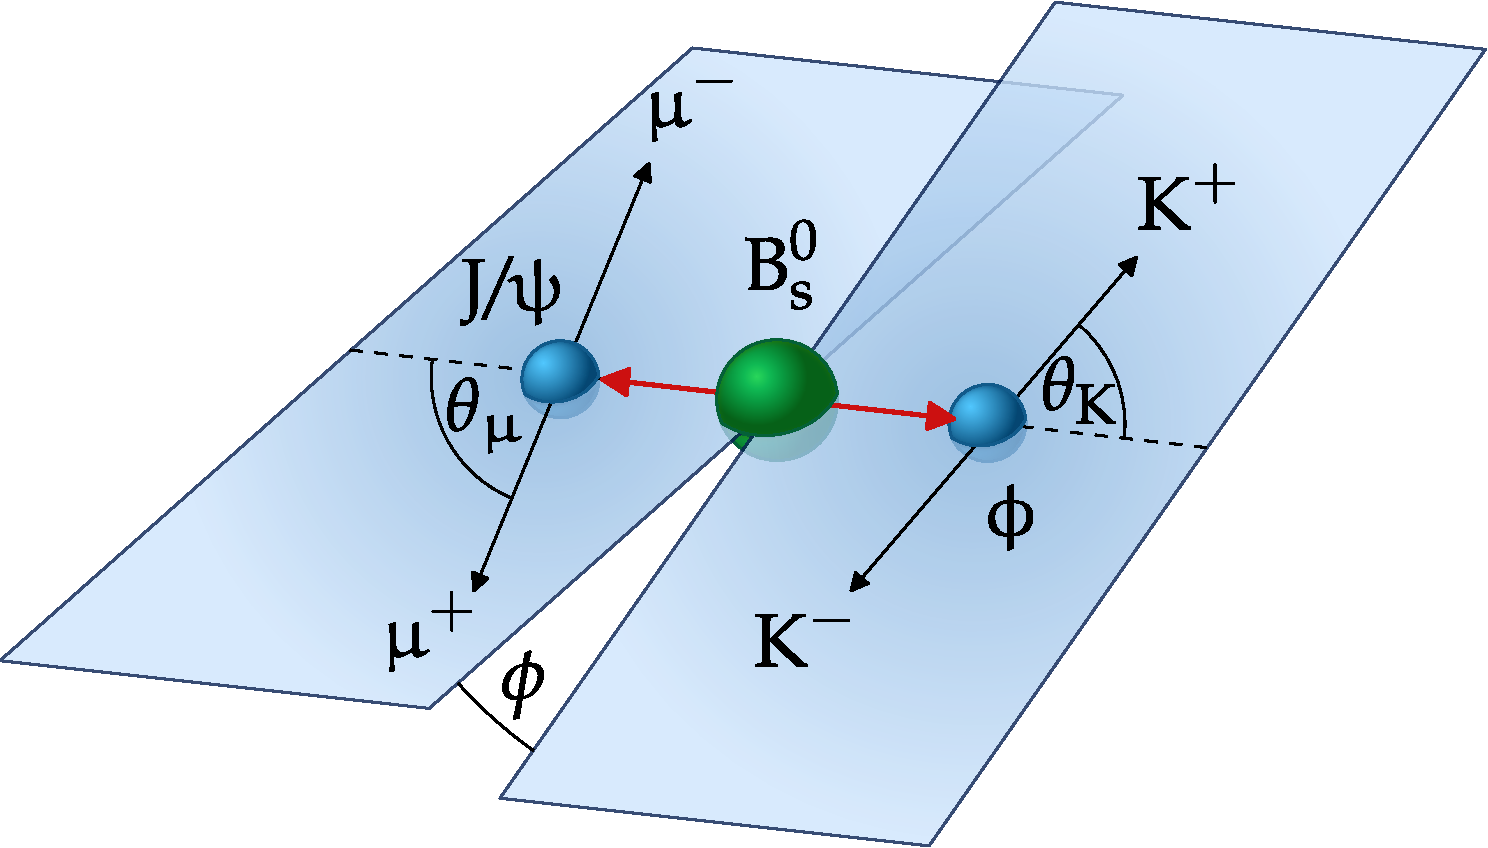
\includegraphics[width=0.7\textwidth]{HelicityPlanes.pdf}
\caption{Definición de los ángulos de helicidad.} \label{fig_angdist}
\end{figure}


Ahora conviene hacer una rotación a la base de las amplitudes de transversalidad, que son
\begin{equation}
\begin{array}{ccl}
\text{S}:& i=1 & \mathcal{A}_{\text{S}} = H_{0,0} \\ \\
  & i=2 & \mathcal{A}_{\perp} = \frac{\sqrt{2}}{2} (H_{1,+1}-H_{1,-1})   \\
\text{P}:& i=3 & \mathcal{A}_{0} = H_{1,0} \\
  & i=4 & \mathcal{A}_{\parallel} = \frac{\sqrt{2}}{2} (H_{1,+1}+H_{1,-1}) \\ \\
  & i=5 & \mathcal{A}_{2\perp} = \frac{\sqrt{2}}{2} (H_{2,+1}-H_{2,-1}) \\
\text{D}:& i=6 & \mathcal{A}_{20} = H_{2,0} \\
  & i=7 & \mathcal{A}_{2\parallel} = \frac{\sqrt{2}}{2} (H_{2,+1}+H_{2,-1})  
\end{array}	\label{eq:amps}
\end{equation}
que se corresponden con estados con autovalores de $\OPcp$ bien definidos. De este modo, la parte angular de la sección eficaz vendría dada por los coeficientes $\Omega_{ij}$ del Apéndice \ref{ap_angdistampana},
\begin{equation}
\frac{d^3 \Gamma}{d\cos\theta_{\text{K}} d\cos\theta_{\upmu} d\phi} \propto \sum_{i=1}^{7}  \sum_{j=1}^i N_{ij} \Omega_{ij}(\theta_{\upmu},\theta_{\text{K}},\phi).
\end{equation}


\begin{table}[H]
\centering
\begin{tabular}{c|ccc} 
\toprule
Onda & $\perp$ & $0$ & $\parallel$\\ 
\midrule
S &      & $-1$ &       \\
P & $-1$ & $+1$ & $+1$  \\
D & $+1$ & $-1$ & $-1$  \\ 
\bottomrule
\end{tabular}
\caption{Signatura, $\eta$, de los autovalores de $\OPcp$ para las amplitudes de transversalidad.}	
\end{table}

\begin{figure}[H]
\centering
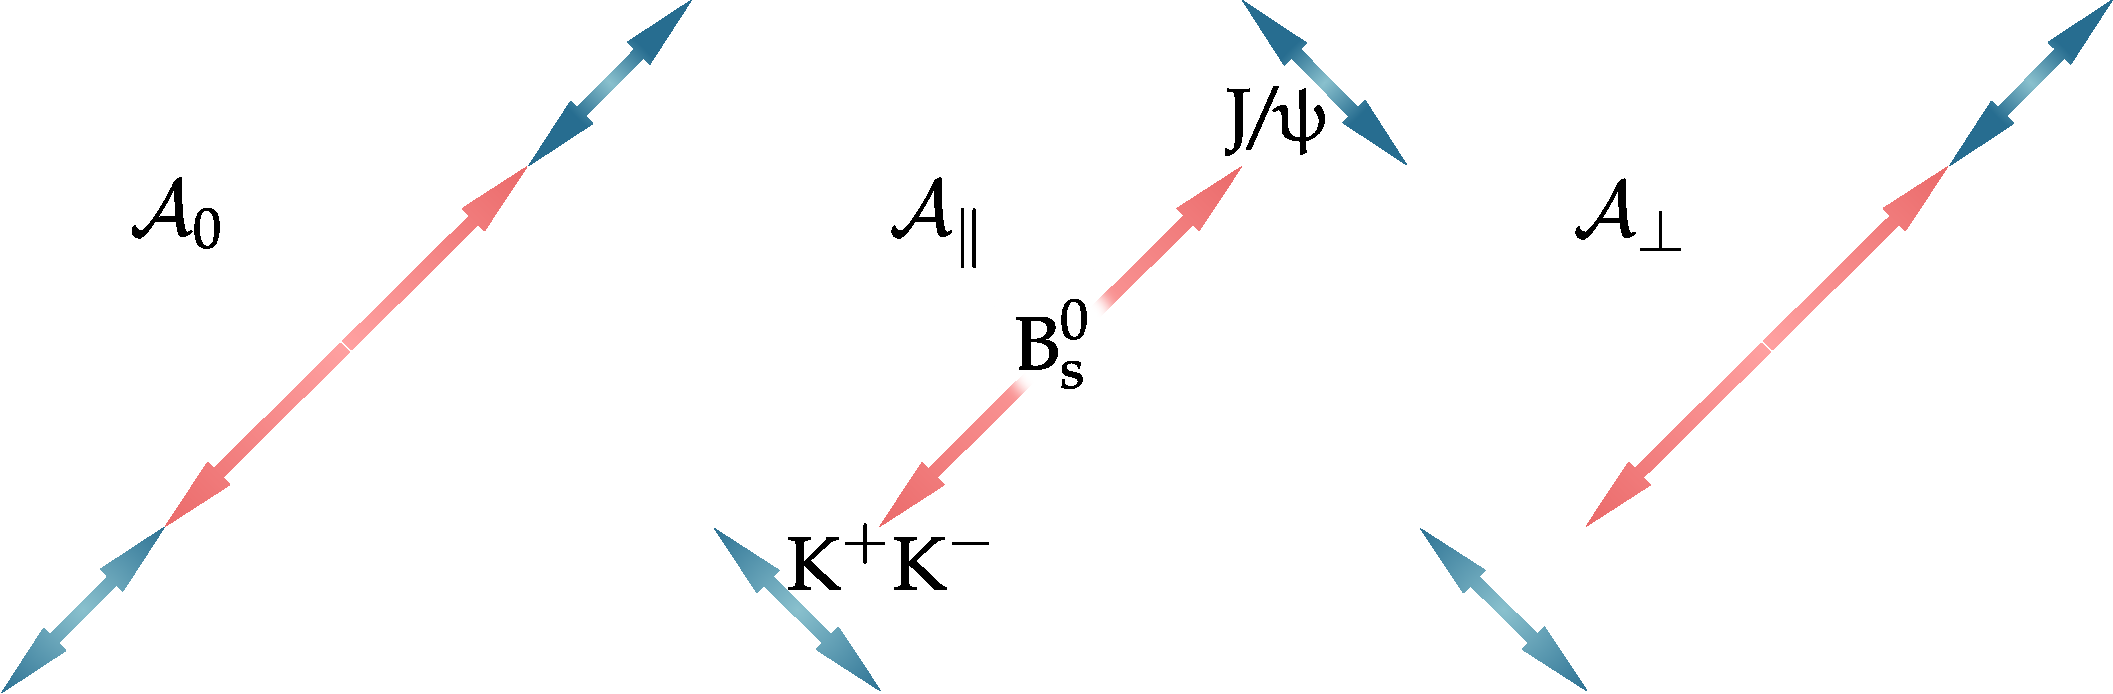
\includegraphics[width=0.8\textwidth]{HelicityPolarizations.pdf}
\caption{Configuraciones de polarización en la base de transversalidad.}
\end{figure}


\subsection{Dependencia temporal} %%%%%%%%%%%%%%%%%%%%%%%%%%%%%%%%%%%%%%%%%%%%%%
\label{sec_tempdist}

Como hemos visto en \S \ref{sec_evotempB}, debido a la mezcla $\Bs-\Bbs$, cada una de las amplitudes de polarización $\mathcal{A}_k$ se describe como
\begin{equation}
\mathcal{A}_k(t) = g_+ (t) \mathcal{A}{}_k^0 + \eta_k \frac{q}{p} g_{-}(t) \overline{\mathcal{A}}{}_f^0
\end{equation}
donde el superíndice $0$ indica que se trata de las amplitudes a $t=0$; $\eta_k$ es el signo del autovalor de $\OPcp$, dependiendo del comportamiento de la amplitud bajo paridad; $p$ y $q$ son parámetros que contiene la física del \emph{mixing}; y las funciones dependientes del tiempo $g_{\pm}(t)$ se corresponden con la Ecuación (\ref{eq_gedete}), verificándose además la relación entre las amplitudes 
\begin{equation}
	\frac{q}{p} \frac{\overline{\mathcal{A}}{}_k^0}{\mathcal{A}{}_k^0} = \eta_k e^{i {\varphi_s}_k}
\end{equation}
con $\varphi_s$ dada por la Ecuación (\ref{eq_phismixdecay}).


Centrándose solo en una contribución $k$, la tasa de desintegración dependiente del tiempo puede expresarse como
\begin{equation}
\begin{split}
\Gamma (t)  \propto e^{-\Gamma t} &\left[\frac{|A|^2+|\overline{A}|^2}{2} \cosh \left(\frac{\Delta \Gamma}{2} t \right) + \frac{|A|^2-|\overline{A}|^2}{2} \cos \left(\Delta m t \right) \right. - \\ & \left. \Re (A^* \overline{A}) \sinh \left(\frac{\Delta \Gamma}{2} t \right) - \Im (A^* \overline{A}) \sinh \left(\Delta m t\right) \right] \\
\overline{\Gamma} (t)  \propto e^{-\Gamma t} &\left[\frac{|A|^2+|\overline{A}|^2}{2} \cosh \left(\frac{\Delta \Gamma}{2} t \right) - \frac{|A|^2-|\overline{A}|^2}{2} \cos \left(\Delta m t \right) \right. - \\ & \left. \Re (A^* \overline{A}) \sinh \left(\frac{\Delta \Gamma}{2} t \right) + \Im (A^* \overline{A}) \sinh \left(\Delta m t\right) \right] 
\end{split}	 \label{eq_decayrateamp}
\end{equation}
o, previa definición de estos coeficientes (\emph{vid.} \ref{ap_angdistampana}),
\begin{equation}
\begin{split}
a_{ij} &= \AmpA_i(0) \AmpA_j^*(0) + \AmpAb_i (0) \AmpAb_j^* (0)\\
b_{ij} &= -\left(\AmpA_i(0) \AmpAb_j^*(0) + \AmpAb_i (0) \AmpA_j^* (0) \right)\\
c_{ij} &= \AmpA_i(0) \AmpA_j^*(0) - \AmpAb_i (0) \AmpAb_j^* (0)\\
d_{ij} &= -i \left(\AmpA_i(0) \AmpAb_j^*(0) - \AmpAb_i (0) \AmpA_j^* (0) \right).
\end{split}
\end{equation}
se puede convenientemente reescribir, para una población inicial de $\Bs$, como
\begin{equation}
	\frac{d\Gamma}{dt} \propto \sum_{i=1}^{7}\sum_{j=1}^i h_{ij}(t)
\end{equation}
donde las funciones dependientes del tiempo, $h_{ij}$, vienen dadas por 
\begin{equation}
\begin{split}
	h_{ij}(t) = e^{-\Gamma t} &\left[  a_{ij} \cosh \left(\frac{\Delta \Gamma}{2} t \right) + c_{ij} \cos \left(\Delta m t \right) \right. + \\ & \left. b_{ij} \sinh \left(\frac{\Delta \Gamma}{2} t \right) + d_{ij} \sinh \left(\Delta m t\right) \right]
\end{split}
\end{equation}
en donde, a la vista de la Ecuación (\ref{eq_decayrateamp}), se puede obtener la expresión para una población inicial de $\Bbs$, cambiando de signo los coeficientes $c_{ij}$ y $d_{ij}$.


Para distinguir mejor los términos susceptibles de violación CP, se escriben las amplitudes
\[\mathcal{A}_f^0 = \sqrt{1-\mathscr{A}_D} \, e^{-i \varphi_D} \, A_f^0, \qquad \overline{\mathcal{A}}_f^0 = \sqrt{1+\mathscr{A}_D} \, e^{i \varphi_D} \, A_f^0 \]
de modo que $\mathscr{A}_D $ es una CPV directa y $\varphi_D$ es una fase débil que da cuenta de la desintegración
\begin{equation}
	\mathscr{A}_D = \frac{|\mathcal{A}_f^0|^2-|\overline{\mathcal{A}}_f^0|^2}{|\mathcal{A}_f^0|^2+|\overline{\mathcal{A}}_f^0|^2}, \qquad \varphi_D = \frac{\text{arg}(\overline{\mathcal{A}}_f^0)-\text{arg}(\mathcal{A}_f^0)}{2}.
\end{equation}
%
La fase de interferencia entre el \textit{mixing} y el \emph{decay} es por tanto,
\begin{equation}
	\varphi_s \equiv \varphi_s^{\Jpsi KK} = \varphi_{M} + 2 \varphi_{D} \label{eq_phismixdecay}
\end{equation}
que junto con $|\lambda|$, son los parámetros que se pretenden medir con precisión en este análisis
\begin{equation}
|\lambda| = \frac{\sqrt{1+\mathscr{A}_D}}{\sqrt{1-\mathscr{A}_D}}	.
\end{equation}





%%%%%%%%%%%%%%%%%%%%%%%%%%%%%%%%%%%%%%%%%%%%%%%%%%%%%%%%%%%%%%%%%%%%%%%%%%%%%%%%
\section{Distribuciones de masa} %%%%%%%%%%%%%%%%%%%%%%%%%%%%%%%%%%%%%%%
% TODO cite ref 22 ananote


Como se decía en la \S \ref{sec_diffrate}, a la hora de parametrizar el espectro de masas en la región del $\fai(1020)$ se usan la propia resonancia $\fai$ de espín $1$ y la contribución de onda S  de espín $0$\footnote{La región de alta masa suele parametrizar $\ftwop$ (de espín $2$), aunque no afecta mucho en la ventana de masa que aquí se emplea.}. A continuación se describen las dependencias de masa junto con los \emph{barrier factors}. \todo{mejor así?}
%
\color{dieg}
En lo sucesivo se tomarán las masas,  $m_{*}$, y anchuras, $\Gamma_{*
}$, como las nominales de la Tabla \ref{tab_massPDG}.


%\color{rem}
%Esto es: $m_{\kaon} = m_{\antikaon} = 493.677$ MeV, $m_{\uppi^+} = m_{\uppi^-} = 139.57018$ MeV, $m_{\text{K}^0} = 497.614$ MeV, $m_{\uppi^0} = 134.9766$ MeV, $m_{\fzero} = 949.9$ MeV, $m_{\ftwop} = 1525$ MeV, $\Gamma_{\ftwop} = 73$ MeV, $m_{\fai} = 1019.4610$, $\Gamma_{\fai} = 4.266$ MeV, $m_{\Bs} = 5366.77$ MeV y $m_{\Jpsi} = 3096.916$ MeV. <CITE PDG>
\color{dieg}

\begin{table}[H]
  \centering
  \begin{tabular}{ccc}
\toprule
Partícula & $m \, (\text{MeV}/c^2)$  & $\Gamma$ \\ \midrule
$\mathrm{K^{\pm}}$    & $ 493.677\pm0.016 $\\
$\mathrm{K^{0}}$      & $497.611\pm0.013$\\
$\uppi^{\pm}$         & $139.57061\pm0.00024$\\
$\uppi^{0}$           & $134.9770\pm0.0005$\\
$\fai (1020)$         & $1019.461\pm0.016$  & $4.249\pm0.013 \, \text{MeV}$\\
$\Jpsi$               & $3096.900\pm0.006$  \\%& $92.9\pm2.8 \,\times 10^{-3}$
$\Bs$                 & $5366.89\pm0.19$ \\ \midrule
$\fzero (980)$        & $949.9\pm2.1$ \\
$\ftwop (1525)$       & $1522_{-3}^{+6}$          & $84_{-8}^{+12} \, \text{keV}$\\
\bottomrule
  \end{tabular}
  \caption{Masas nominales de partículas tomados de \cite[primer bloque]{pdg2018} y \cite[segundo bloque]{Aaij:1664567}.} \label{tab_massPDG}
\end{table}
\color{norm}


\color{new}
La amplitud $R(m)$ se usa para describir la \emph{line--shape} de masa de la resonancia $R$, en este caso correspondientes a $\fzero$, $\fai$ y $\ftwop$. Se combina esta función con las propiedades del decaimiento del $\Bs$, resultando la expresión \cite{Aaij:1664567}  
\begin{equation}
  \mathcal{M}_R = \sqrt{2 j + 1}\, \sqrt{q_m,q_{\Bs}} \,\mathfrak{B}_j \, R(m) \label{eq:masslineshape}
\end{equation}
siendo $j$ el espín de la resonancia, $\mathfrak{B}_j$ los \emph{barrier factors} y  $\sqrt{q_m,q_{\Bs}}$ el factor de espacio fásico, para tener en cuenta la cinemática de la desintegración a cuatro cuerpos se tiene que incluir una densidad de espacio fásico.
%
%TODO <meter algo más de palla>
%
%
% P
%
%
\color{norm}
%
El espacio fásico va a depender de los momentos $q_{\kaon}$  ($q_{\antikaon}$), momento del $\kaon$($\antikaon$) respecto del sistema en reposo $\antikaon\kaon$; y  $q_{\Bs}$, momento del sistema $\antikaon\kaon$ respecto del sistema en reposo del $\Bs$. Todos esos momentos se construyen de la forma:
\begin{equation}
q_m \equiv q(m,m_1,m_2) = \frac{1}{2}  \sqrt{m^2+\frac{\left(m_1^2-m_2^2\right){}^2}{m^2}-2 \left(m_1^2+m_2^2\right)}	
\end{equation}
y por lo tanto se definen $q_m \equiv q(m_R,m_{\kaon},m_{\antikaon})$, donde $m_R$ es la masa de la resonancia, y $q_{\Bs} \equiv q(m_{\Bs},m,m)$.



Los \emph{barrier factors} de momento angular se construyen como \cite{blatt2012theoretical}
\begin{equation}
\mathfrak{B}_j = \left[ B_{\ell}(q_{\Bs},\tilde{q}_{\antikaon\kaon}) \left( \frac{q_{\Bs}}{\tilde{q}_{\antikaon\kaon}} \right)^{\ell}\right] \, \left[ B_j(q_m,\tilde{q}_m) \left( \frac{q_m}{\tilde{q}_m} \right)^j\right]
\end{equation}
siendo $B_j(q,q0) \equiv B(j,q,q_0)$ los Blatt--Weisskopf \emph{barrier factors}, que hasta $j=2$ son:
\begin{equation} 
B_0 = 1, \qquad B_1 = \sqrt{\frac{1+(q_0d)^2}{1+(qd)^2}}, \qquad B_2 = \sqrt{\frac{9+3(q_0d)^2+(q_0d)^4}{9+3(qd)^2+(qd)^4}},
\end{equation}
donde el parámetro $d$ se corresponde con el tamaño característico de la partícula que decae y se mantiene fijo en $d = \frac{3\times10^{-3}}{j}$.



Para cada una de las contribuciones se emplea una resonancia $R(m)$, para lo que se hace uso de las siguientes distribuciones \cite{paperPhis}:

\paragraph{Distribución de Breit--Wigner}

Tanto la resonancia $\fai(1020)$, vectorial, como $\ftwop(1525)$, tensorial, se parametrizan con una función Breit--Wigner relativista que se define como: 
\begin{equation}
\mathcal{B}(m;m_0,\Gamma_0,m_1,m_2,j) = \frac{1}{(m_0^2-m^2)-im_0\Gamma(m;m_0,\Gamma_0,m_1,m_2,j)}
\end{equation}
La función $\Gamma(m;m_0,\Gamma_0,m_1,m_2,j)$, llamada \emph{running width}, viene dada por
\begin{equation}
	\Gamma(m;m_0,\Gamma_0,m_1,m_2,j) = \Gamma_0 \left(\frac{q_m}{q_0}\right)^{2j+1}\, \frac{m_0}{m} \, B_j (q_m,q_0)
\end{equation}


\paragraph{Distribución de Flatté}

Para la resonancia $\fzero(980)$, escalar,  se parametriza con una función Breit--Wigner relativista modificada, denominada distribución de Flatté, definida tal que así: 
\begin{equation}
\mathcal{F}(m;m_0) = \frac{1}{(m_0^2-m^2)-im_0(\Gamma_\text{K}+\Gamma_{\uppi})}
\end{equation}
siendo,
\begin{equation}
	\Gamma_{\text{K}} = \sqrt{1-\frac{m_{\text{K}}^2}{m^2}}, \qquad 	\Gamma_{\uppi} = \sqrt{1-\frac{m_{\uppi}^2}{m^2}}.
\end{equation}
La masa del polo del $\fzero(980)$ está muy cerca del umbral cinemático para decaer en dos kaones. Debido a las condiciones de unitariedad, este efecto distorsiona significativamente la forma del $\fzero$ en el espectro de masa de dos piones \cite{baru2005flatte}. \todo{qué tal así?}




%%%%%%%%%%%%%%%%%%%%%%%%%%%%%%%%%%%%%%%%%%%%%%%%%%%%%%%%%%%%%%%%%%%%%%%%%%%%%%%%
\subsection{Contribuciones de masa}

El espectro de masa $M_{\text{KK}}$ estará formado a lo sumo por tres componentes que se construirán con Ecuación \ref{eq:masslineshape} y los parámetros de la Tabla \ref{tab_massPDG}. Las formas de las ditribuciones y sus fases pueden verse en la Figura \ref{fig:masslineshape}, donde pueden apreciarse diferentes contribuciones dependiendo del la masa.

%TODO amañar pictures con python
\begin{figure}[H]
\centering
\subfloat[Resonancia de la masa $\fzero$ (azul) y distribución de la fase (verde).\label{fig_flatte}]{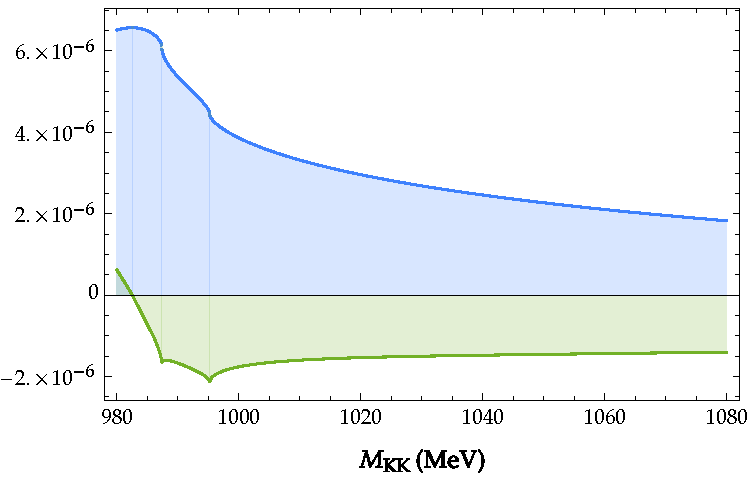
\includegraphics[width=0.48\textwidth]{flatte.pdf}} \hfill
\subfloat[Resonancia de la masa $\fai$ (azul) y distribución de la fase (verde).\label{fig_faires}]{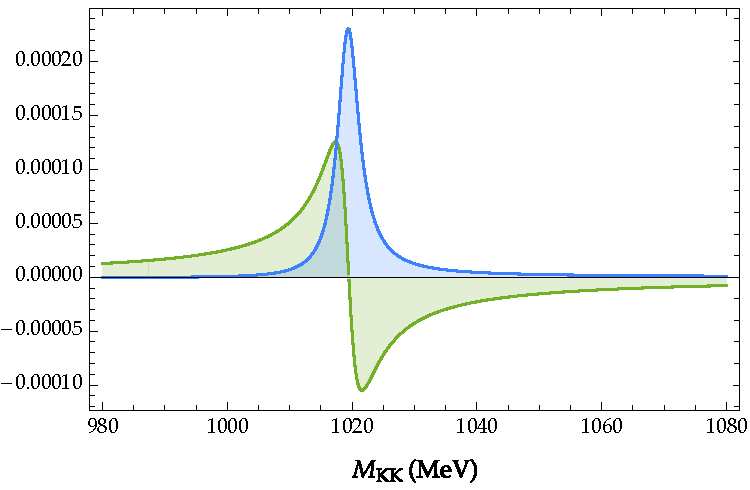
\includegraphics[width=0.48\textwidth]{BW_phi.pdf}} \hfill
\subfloat[Resonancia de la masa $\ftwop$ (azul) y distribución de la fase (verde).\label{fig_f2pres}]{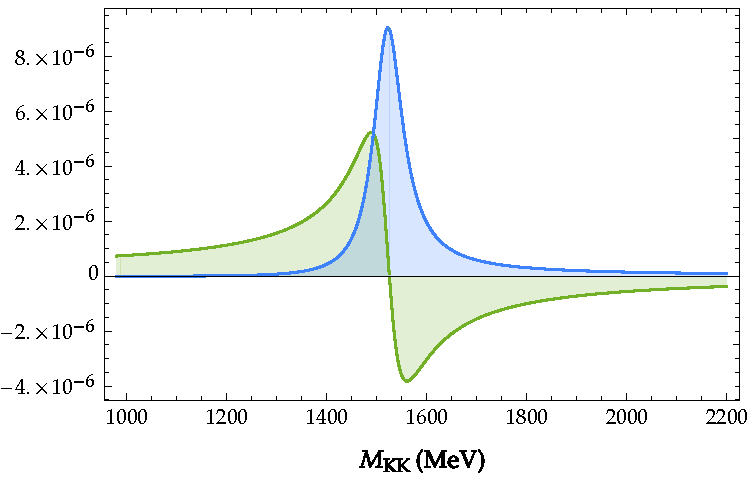
\includegraphics[width=0.48\textwidth]{BW_f2p.pdf}} \hfill
\subfloat[Espectro de masa KK con las resonacias $\fzero$ (naranja), $\fai$ (azul) y $\ftwop$ (rojo). Se hace uso de la escala logarítmica para poder distinguir las tres formas. \label{fig_mKK_linemass}]{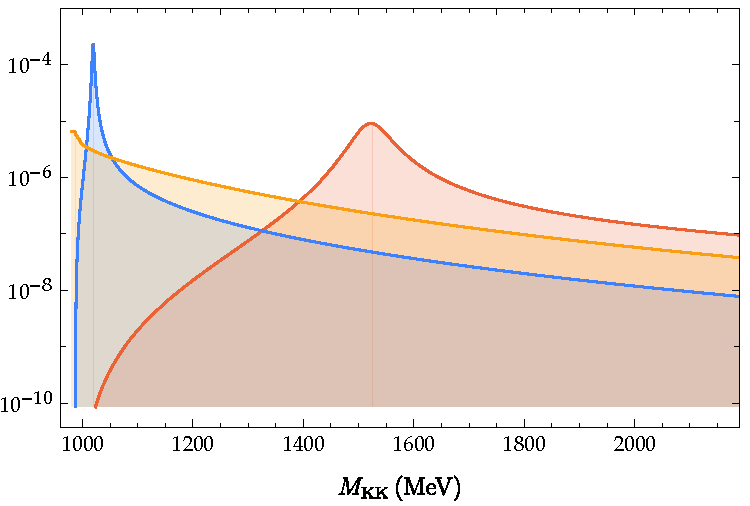
\includegraphics[width=0.48\textwidth]{mass_shape.pdf}} \hfill
\caption{Funciones de distribución de masa, para las 3 componentes resonantes estudiadas.}  \label{fig:masslineshape}
\end{figure}

\paragraph{Componente escalar $\text{(\textit{j}}\text{=}\text{0)}$}
Esta componente se supone la dominante en los rangos de masa $980- 1000$ MeV$/c^2$ y $1050-1400$ MeV$/c^2$ y se atribuye a una contribución de onda S resonante, correspondiente con el $\fzero(980)$. %, aunque también existe la posibilidad de añadir  S--\emph{wave}  no resonante.
La ausencia de un completo entendimiento de esta componente y de su relación con la la onda P, provoca que se haga un ajuste en diferentes bines de masa (\emph{vid.} \S \ref{sec_factorescspcspdcssd}). Esta componente se modela con una forma \todo{???}
\begin{equation}
	s(m) = \mathcal{F}(m;m_{\fzero}) \, \mathfrak{B}_0.
\end{equation}

\paragraph{Componente vectorial $\text{(\textit{j}}\text{=}\text{1)}$}
La componente principal de la ventana de masa es la correspondiente al $\fai(1020)$ de espín $1$. Para su modelado se emplea una Breit--Wigner relativista, quedando su \emph{line--shape}
\begin{equation}
	p(m) = \mathcal{B}(m;m_{\fai},\Gamma_{\fai},m_{\kaon},m_{\antikaon},1) \, \mathfrak{B}_1.
\end{equation}
Es la componente mayoritaria en el rango de masa $1000-1050$ MeV$/c^2$.


\paragraph{Componente tensorial $\text{(\textit{j}}\text{=}\text{2)}$}
A pesar de que esta contribución es despreciable en la ventana de masa $[980,1200]$ MeV, la resonancia $\ftwop(1525)$ de espín $2$ también hace uso de una BW,
\begin{equation}
	d(m) = \mathcal{B}(m;m_{\ftwop},\Gamma_{\ftwop},m_{\kaon},m_{\antikaon},1) \, \mathfrak{B}_2.
\end{equation}
Su preeminencia se sitúa en el rango de masa $1400-2200$ MeV$/c^2$.




%%%%%%%%%%%%%%%%%%%%%%%%%%%%%%%%%%%%%%%%%%%%%%%%%%%%%%%%%%%%%%%%%%%%%%%%%%%%%%%%
%\subsection[ee]{Factores 
%\begingroup
%\fontfamily{newtxsf}\selectfont\bfseries\sffamily\sansmath
%$C_{\text{SP}}$, $\bm{C_{\text{SD}}}$ y $\bm{C_{\text{PD}}}$
%\endgroup
%} %%%%%%

\subsection{Factores 
$\text{\textit{C}}_{\text{SP}}$, $\text{\textit{C}}_{\text{SD}}$ y $\text{\textit{C}}_{\text{PD}}$
}

\label{sec_factorescspcspdcssd}
%TODO bold math

En la Tabla \ref{tab_coeffsfk}, a las contribuciones correspondientes a interferencia entre las amplitudes, las acompañan los factores $C_{\text{SP}}$, $C_{\text{SD}}$ y $C_{\text{PD}}$ , que dan cuenta del cambio relativo de fracciones de las diferentes polarizaciones en los bines de masa $m_{\text{KK}}$.

Para poder calcular estos factores, se deben explicitar las expresiones analíticas de las funciones de forma normalizadas de la masas  $s(m_{\text{KK}})$ (onda S), $p(m_{\text{KK}})$ (onda P)  y $d(m_{\text{KK}})$ (onda D). El problema nace principalmente porque $\langle p \times s^* \rangle \neq \langle p \rangle \langle s^* \rangle$ (e igual para los demás factores) \cite{Xie:1461783}. Entonces para cada bin $m_{\text{KK}}$, se integra  
\begin{equation}
C_{\text{SP}} e^{-i \theta_{\text{SP}}} =
\frac{\int_{m_{KK}^L}^{m_{KK}^H} { p(m_{KK}) \times s(m_{KK})^*} \:\:d m_{KK}}
{\sqrt{\int_{m_{KK}^L}^{m_{KK}^H} { |p(m_{KK})|^2}  \:\:d m_{KK} \,\,\int_{m_{KK}^L}^{m_{KK}^H} { |s(m_{KK})|^2}  \:\:d m_{KK}}}
\end{equation}
y análogamente para los demás factores de corrección.
\todo{more on this?}


\begin{table}[H]
\centering
\begin{tabular}{c|c}
\toprule
$m_{\text{KK}}$ GeV & $C_{\text{SP}}$ \\ \midrule
$[0.990,1.008]$ & 0.8463  \\
$(1.008,1.016]$ & 0.8756  \\
$(1.016,1.020]$ & 0.8478  \\
$(1.020,1.024]$ & 0.8833  \\
$(1.024,1.032]$ & 0.9415  \\
$(1.032,1.050]$ & 0.9756  \\
\bottomrule
\end{tabular}
\caption{Factores de corrección para los bines de masa KK definidos en la región del $\fai(1020)$.}	
\end{table}


\begin{table}[H]
\centering
\begin{tabular}{c|ccc}
\toprule
$m_{\text{KK}}$ GeV & $C_{\text{SP}}$ & $C_{\text{SD}}$ & $C_{\text{PD}}$\\ \midrule
$[1.0,1.2]$ & 0.8420 & 0.8525 & 0.9965 \\
$(1.2,1.4]$ & 0.9273 & 0.9925 & 0.9623 \\
$(1.4,1.6]$ & 0.9053 & 0.9987 & 0.9122 \\
$(1.6,1.8]$ & 0.9485 & 0.9990 & 0.9372 \\
$(1.8,2.0]$ & 0.9734 & 0.9969 & 0.9531 \\
$(2.0,2.2]$ & 0.9840 & 0.9901 & 0.9499 \\
\bottomrule
\end{tabular}
\caption{Factores de corrección para los bines de masa KK definidos en la ventana de masa $[1.0,2.2]$ GeV$/c^2$.}	
\end{table}





%%%%%%%%%%%%%%%%%%%%%%%%%%%%%%%%%%%%%%%%%%%%%%%%%%%%%%%%%%%%%%%%%%%%%%%%%%%%%%%%
%%%%%%%%%%%%%%%%%%%%%%%%%%%%%%%%%%%%%%%%%%%%%%%%%%%%%%%%%%%%%%%%%%%%%%%%%%%%%%%%
%%%%%%%%%%%%%%%%%%%%%%%%%%%%%%%%%%%%%%%%%%%%%%%%%%%%%%%%%%%%%%%%%%%%%%%%%%%%%%%%

\bigskip

\begin{center}
	$***$
\end{center}

\medskip

%%%%%%%%%%%%%%%%%%%%%%%%%%%%%%%%%%%%%%%%%%%%%%%%%%%%%%%%%%%%%%%%%%%%%%%%%%%%%%%%
%%%%%%%%%%%%%%%%%%%%%%%%%%%%%%%%%%%%%%%%%%%%%%%%%%%%%%%%%%%%%%%%%%%%%%%%%%%%%%%%
%%%%%%%%%%%%%%%%%%%%%%%%%%%%%%%%%%%%%%%%%%%%%%%%%%%%%%%%%%%%%%%%%%%%%%%%%%%%%%%%

\begin{subappendices}

%\titleformat{\section} 
%  {\normalfont}{\spacedlowsmallcaps\appendixname\ %
%  {\spacedallcaps\thesection}}%
%  {1em}{\spacedallcaps}

%%%%%%%%%%%%%%%%%%%%%%%%%%%%%%%%%%%%%%%%%%%%%%%%%%%%%%%%%%%%%%%%%%%%%%%%%%%%%%%%



%%%%%%%%%%%%%%%%%%%%%%%%%%%%%%%%%%%%%%%%%%%%%%%%%%%%%%%%%%%%%%%%%%%%%%%%%%%%%%%%
%Matrices Wigner
%%%%%%%%%%%%%%%%%%%%%%%%%%%%%%%%%%%%%%%%%%%%%%%%%%%%%%%%%%%%%%%%%%%%%%%%%%%%%%%%
%%%%%%%%%%%%%%%%%%%%%%%%%%%%%%%%%%%%%%%%%%%%%%%%%%%%%%%%%%%%%%%%%%%%%%%%%%%%%%%%
%%%%%%%%%%%%%%%%%%%%%%%%%%%%%%%%%%%%%%%%%%%%%%%%%%%%%%%%%%%%%%%%%%%%%%%%%%%%%%%%
\section{Matrices de Wigner}
\label{app_matwig}
%%%%%%%%%%%%%%%%%%%%%%%%%%%%%%%%%%%%%%%%%%%%%%%%%%%%%%%%%%%%%%%%%%%%%%%%%%%%%%%%
%%%%%%%%%%%%%%%%%%%%%%%%%%%%%%%%%%%%%%%%%%%%%%%%%%%%%%%%%%%%%%%%%%%%%%%%%%%%%%%%
%%%%%%%%%%%%%%%%%%%%%%%%%%%%%%%%%%%%%%%%%%%%%%%%%%%%%%%%%%%%%%%%%%%%%%%%%%%%%%%%



%%%%%%%%%%%%%%%%%%%%%%%%%%%%%%%%%%%%%%%%%%%%%%%%%%%%%%%%%%%%%%%%%%%%%%%%%%%%%%%%
%\section{Introducción } %%%%%%%%%%%%%%%%%%%%%%%%%%%%%%%%%%%%%%%%%%%%%%%%%%%%%%%%

Se denominan funciones $D$ de Wigner, $D_{m,m'}^j(\alpha,\beta,\gamma)$, a los elementos de matriz del operador de rotaciones, $R(\alpha,\beta,\gamma)$, para un estado $|j\,m\rangle$ con valores bien definidos de momento angular $j^2$ y de su proyección $j_z$ \cite{kutschke1996angular}. De modo que
\begin{equation}
	\psi_{jm'}(\theta',\phi',\sigma') = R(\Omega) \psi_{jm} (\theta,\phi,\sigma) = \sum_{m' = -j}^j  \psi_{jm} (\theta,\phi,\sigma) D_{m,m'}^j(\Omega),
\end{equation}
siendo $\theta$ y $\phi \, (\theta'$ y $\phi')$ los ángulos polares iniciales (rotados) y $\sigma(\sigma')$ referida a las variables de espín. Además, se tiene la relación con las matrices $d$ de Wigner,
\begin{equation}
	D_{m,m'}^j (\alpha,\beta,\gamma) \equiv e^{-i\alpha m} d_{m,m'}^j (\beta) e^{-i\gamma m'}.
\end{equation}


Al considerar la desintegración del $\Bs$ en $\Jpsi$ y $\fai$, que a su vez decaen en $\muon \antimuon$ y  $\kaon \antikaon$ \footnote{Aunque los nombres de partículas sean específicos, este es un marco y procedimiento general para las desintegraciones a cuatro cuerpos que mediados por dos resonancias intermedias para desintegraciones escalares.}.
%
Los estados para las partículas se definen, por ejemplo, para el $\Jpsi$, como $\Jpsi:  |j_{\Jpsi} \,\lambda_{\Jpsi}\rangle$. Cuando $\Jpsi$ decae, se proyecta en un nuevo plano, $X_{\Jpsi}',Y_{\Jpsi}',Z_{\Jpsi}'$, cuya amplitud es proporcional a 
\begin{equation*}
\langle j_{\Jpsi},\, \lambda_{\muon} - \lambda_{\antimuon} | R(\alpha,\beta,\gamma) | j_{\Jpsi} , \lambda_{\Jpsi} \rangle \equiv D_{\lambda_{\Jpsi},\lambda_{\muon} - \lambda_{\antimuon}}^{j_{\Jpsi}}	(\alpha,\beta,\gamma)
\end{equation*}
es decir, precisamente la matriz de Wigner-$D$. Aquí $\alpha,\beta$ y $\gamma$
son los ángulos de Euler, que en la Mecánica Clásica  definen cualquier posible rotación en el espacio tridimensional. Hay otras convenciones posibles para estos ángulos, una de ellas --- y la usada por \lhcb --- es la convención de Jacobi--Wick \cite{kutschke1996angular}, que dicta
$R(\alpha,\beta,\gamma)  \rightarrow R(\alpha,\beta,-\alpha).  $


\begin{figure}[H]
\centering
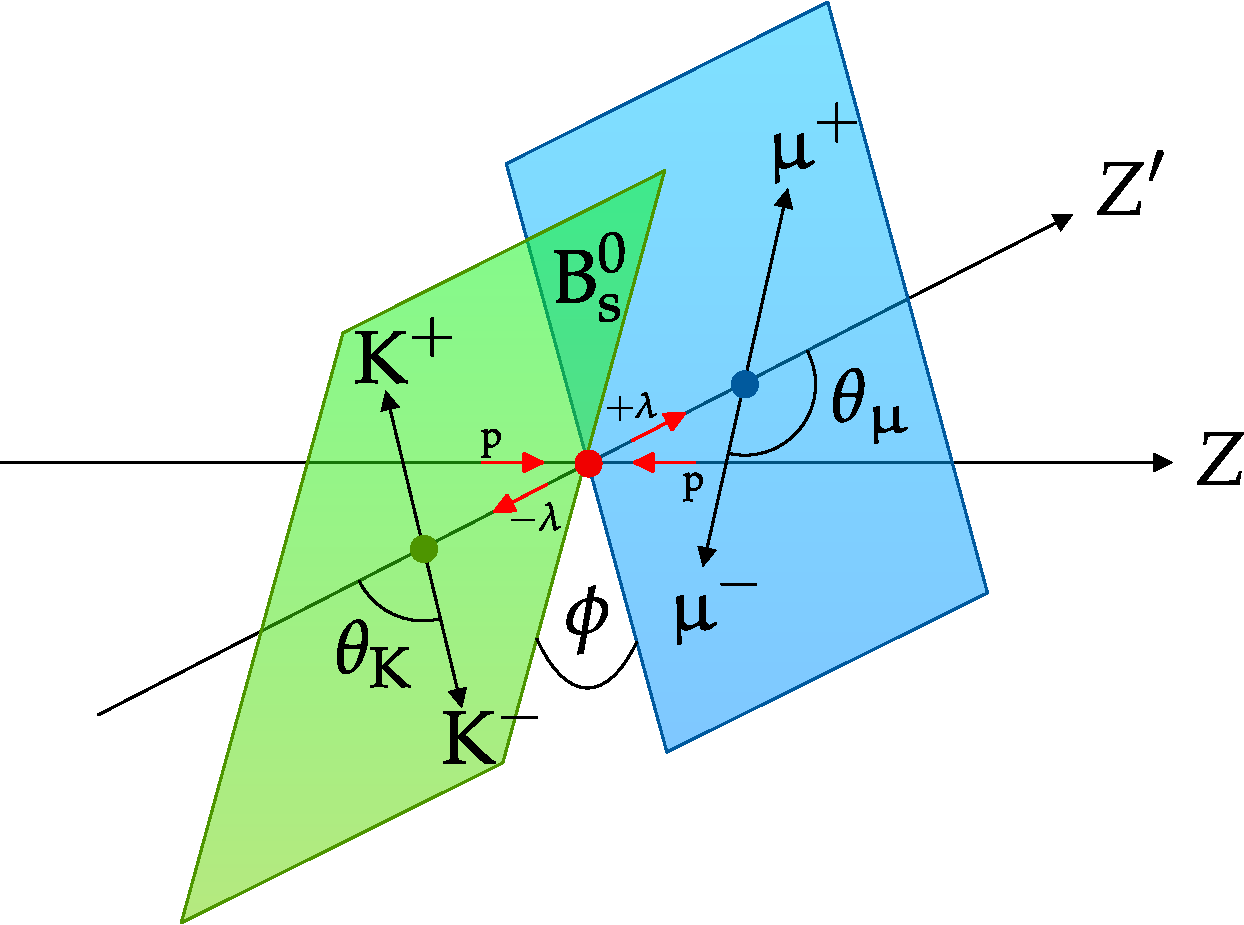
\includegraphics[width=0.48\textwidth]{WignerD1}
\hfill
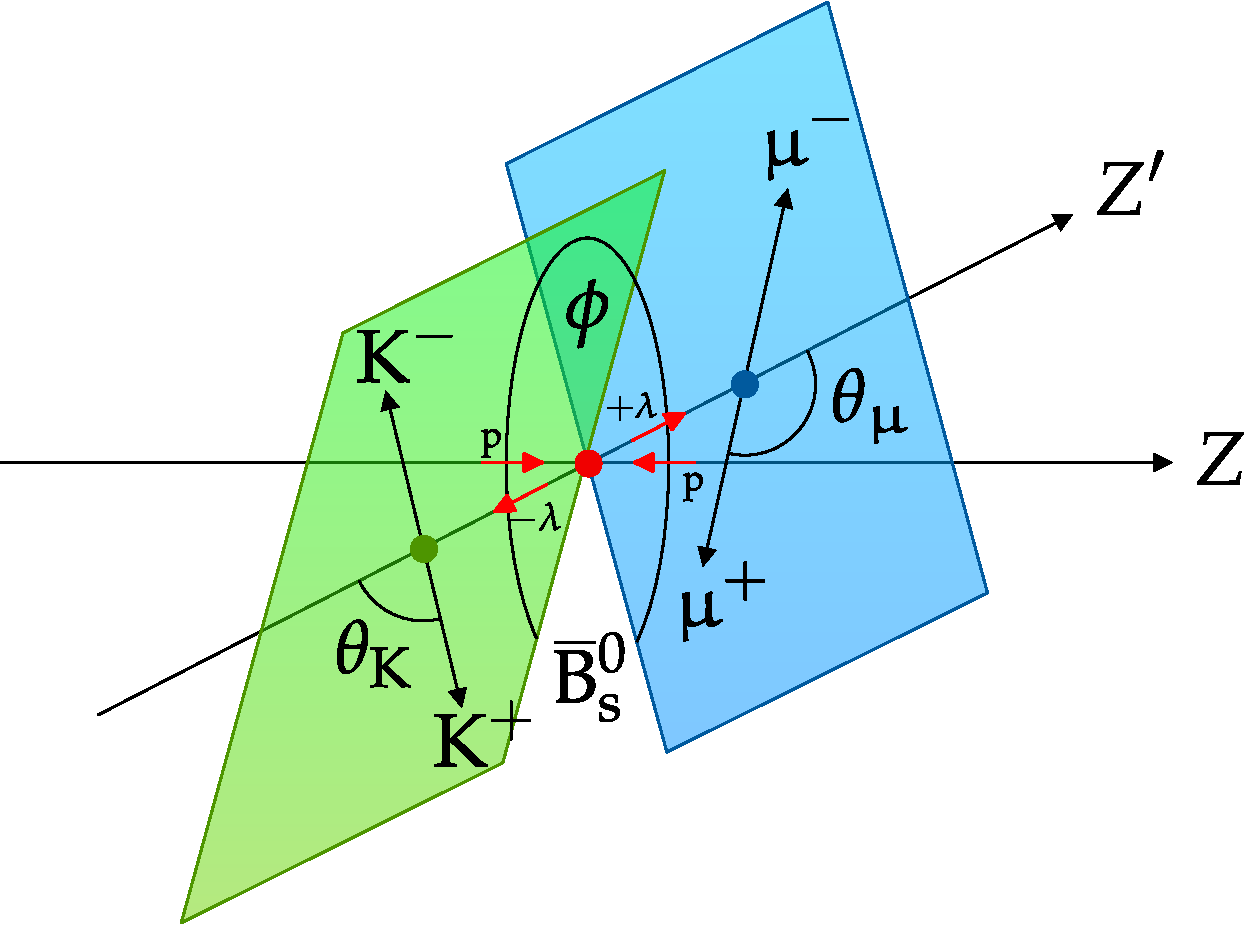
\includegraphics[width=0.48\textwidth]{WignerD2}
\caption{Definición de la helicidad y ángulos de helicidad para los desintegraciones $\Bs$ y $\Bbs$.}	
\end{figure}



%
Por tanto, la amplitud del proceso será proporcional al siguiente producto de funciones de Wigner
\[\mathcal{A} \sim D_{\lambda_{\Bs},\lambda_{\Jpsi}-\lambda_{\fai}}^{j_{\Bs}}\,D_{\lambda_{\Jpsi},\lambda_{\muon}-\lambda_{\antimuon}}^{j_{\Jpsi}}\, D_{\lambda_{\fai},\lambda_{\kaon}-\lambda_{\antikaon}}^{j_{\fai}}\]
Dado que el $\Bs$ carece de espín, $D_{0,\lambda_{\Jpsi}-\lambda_{\fai}}^0 = \delta_{0,\lambda_{\Jpsi}-\lambda_{\fai}}^0$, por lo que las helicidades del $\Jpsi$ y del $\fai$ deben ser contrarias respecto de la dirección del $\Bs$ (o equivalentemente, conservar el momento lineal). Así,
\[\mathcal{A} \sim D_{\lambda_{\Jpsi},\lambda_{\muon}-\lambda_{\antimuon}}^{j_{\Jpsi}}\, D_{\lambda_{\fai},\lambda_{\kaon}-\lambda_{\antikaon}}^{j_{\fai}},\]
o denominando $\lambda \equiv \lambda_{\Jpsi} = - \lambda_{\fai} $, $\alpha = \lambda_{\muon}-\lambda_{\antimuon}$, $j \equiv j_{\fai}$ y como los kaones son escalares \cite{zhang2013time},
\begin{equation}
\begin{split}
\mathcal{A} &  \sim D_{\lambda,\alpha}^{1}(0, \theta_{\upmu}, 0)\, D_{-\lambda,0}^{j} (\phi, \theta_{\text{K}} , -\phi ) = \\
&= d_{\lambda,\alpha}^{1} (\theta_{\upmu})\, e^{-i (-\lambda) (\phi)} d_{-\lambda,0}^{j}(\theta_{\text{K}}) e^{-i (0) (-\phi)} = \\ 
&= e^{i\lambda \phi} \,d_{\lambda,\alpha}^{1} (\theta_{\upmu})\,  d_{-\lambda,0}^{j}(\theta_{\text{K}}) .
\end{split}	
\end{equation}
encontrando así la notación estándar de los términos angulares de la amplitud.



%%%%%%%%%%%%%%%%%%%%%%%%%%%%%%%%%%%%%%%%%%%%%%%%%%%%%%%%%%%%%%%%%%%%%%%%%%%%%%%%
%%%%%%%%%%%%%%%%%%%%%%%%%%%%%%%%%%%%%%%%%%%%%%%%%%%%%%%%%%%%%%%%%%%%%%%%%%%%%%%%
%%%%%%%%%%%%%%%%%%%%%%%%%%%%%%%%%%%%%%%%%%%%%%%%%%%%%%%%%%%%%%%%%%%%%%%%%%%%%%%%



%%%%%%%%%%%%%%%%%%%%%%%%%%%%%%%%%%%%%%%%%%%%%%%%%%%%%%%%%%%%%%%%%%%%%%%%%%%%%%%%
\section{Coeficientes del análisis angular de amplitudes}
\label{ap_angdistampana}

Se presentan en forma de tabla los coeficientes de la sección eficaz diferencial desarrollada en el Capítulo \ref{cha:pheno}.




\begin{table}
\centering
\begin{tabular}{LC}
\toprule
\multicolumn{1}{c}{$N_{ij}$} & \Omega_{ij} \\
\midrule
\phantom{C_{\mathrm{SP}}} A_{\text{S}}^2 & \frac{1}{3} \sin ^2\left(\theta _{\mu }\right) \\
 C_{\mathrm{SP}} A_{\text{S}} A_{\perp} & \frac{\sin (\phi ) \sin \left(\theta _K\right) \sin \left(2 \theta _{\mu }\right)}{\sqrt{6}} \\
 \phantom{C_{\mathrm{SP}}} A_{\perp}^2 & \frac{1}{2} \left(\cos ^2(\phi )+\cos ^2\left(\theta _{\mu }\right) \sin ^2(\phi )\right) \sin ^2\left(\theta _K\right) \\
 C_{\mathrm{SP}} A_{\text{S}} A_{0} & \frac{2 \cos \left(\theta _K\right) \sin ^2\left(\theta _{\mu }\right)}{\sqrt{3}} \\
 \phantom{C_{\mathrm{SP}}} A_{\perp} A_{0} & -\frac{\sin (\phi ) \sin \left(2 \theta _K\right) \sin \left(2 \theta _{\mu }\right)}{2 \sqrt{2}} \\
 \phantom{C_{\mathrm{SP}}} A_{0}^2 & \cos ^2\left(\theta _K\right) \sin ^2\left(\theta _{\mu }\right) \\
 C_{\mathrm{SP}} A_{\text{S}} A_{\parallel} & \frac{\cos (\phi ) \sin \left(\theta _K\right) \sin \left(2 \theta _{\mu }\right)}{\sqrt{6}} \\
 \phantom{C_{\mathrm{SP}}} A_{\perp} A_{\parallel} & \frac{1}{2} \sin (2 \phi ) \sin ^2\left(\theta _K\right) \sin ^2\left(\theta _{\mu }\right) \\
 \phantom{C_{\mathrm{SP}}} A_{0} A_{\parallel} & \frac{\cos (\phi ) \sin \left(2 \theta _K\right) \sin \left(2 \theta _{\mu }\right)}{2 \sqrt{2}} \\
 \phantom{C_{\mathrm{SP}}} A_{\parallel}^2 & \frac{1}{2} \left(\cos ^2(\phi ) \cos ^2\left(\theta _{\mu }\right)+\sin ^2(\phi )\right) \sin ^2\left(\theta _K\right) \\
 C_{\mathrm{SD}} A_{\text{S}} A_{2\perp} & \frac{1}{2} \sqrt{\frac{5}{6}} \sin (\phi ) \sin \left(2 \theta _K\right) \sin \left(2 \theta _{\mu }\right) \\
 C_{\mathrm{PD}} A_{\perp} A_{2\perp} & \frac{1}{2} \sqrt{5} \left(\cos ^2(\phi )+\cos ^2\left(\theta _{\mu }\right) \sin ^2(\phi )\right) \sin \left(\theta _K\right) \sin \left(2 \theta _K\right) \\
 C_{\mathrm{PD}} A_{0} A_{2\perp} & \sqrt{\frac{5}{2}} \cos ^2\left(\theta _K\right) \sin (\phi ) \sin \left(\theta _K\right) \sin \left(2 \theta _{\mu }\right) \\
 C_{\mathrm{PD}} A_{\parallel} A_{2\perp} & -\frac{1}{2} \sqrt{5} \cos \left(\theta _K\right) \sin (2 \phi ) \sin ^2\left(\theta _K\right) \sin ^2\left(\theta _{\mu }\right) \\
 \phantom{C_{\mathrm{SP}}} A_{2\perp}^2 & \frac{5}{8} \left(\cos ^2(\phi )+\cos ^2\left(\theta _{\mu }\right) \sin ^2(\phi )\right) \sin ^2\left(2 \theta _K\right) \\
 C_{\mathrm{SD}} A_{\text{S}} A_{20} & \frac{1}{6} \sqrt{5} \left(3 \cos \left(2 \theta _K\right)+1\right) \sin ^2\left(\theta _{\mu }\right) \\
 C_{\mathrm{PD}} A_{\perp} A_{20} & -\frac{1}{4} \sqrt{\frac{5}{6}} \left(3 \cos \left(2 \theta _K\right)+1\right) \sin (\phi ) \sin \left(\theta _K\right) \sin \left(2 \theta _{\mu }\right) \\
 C_{\mathrm{PD}} A_{0} A_{20} & \frac{1}{2} \sqrt{\frac{5}{3}} \cos \left(\theta _K\right) \left(3 \cos \left(2 \theta _K\right)+1\right) \sin ^2\left(\theta _{\mu }\right) \\
 C_{\mathrm{PD}} A_{\parallel} A_{20} & \frac{1}{4} \sqrt{\frac{5}{6}} \cos (\phi ) \left(3 \cos \left(2 \theta _K\right)+1\right) \sin \left(\theta _K\right) \sin \left(2 \theta _{\mu }\right) \\
 \phantom{C_{\mathrm{SP}}} A_{2\perp} A_{20} & -\frac{5 \left(3 \cos \left(2 \theta _K\right)+1\right) \sin (\phi ) \sin \left(2 \theta _K\right) \sin \left(2 \theta _{\mu }\right)}{8 \sqrt{6}} \\
 \phantom{C_{\mathrm{SP}}} A_{20}^2 & \frac{5}{48} \left(3 \cos \left(2 \theta _K\right)+1\right){}^2 \sin ^2\left(\theta _{\mu }\right) \\
 C_{\mathrm{SD}} A_{\text{S}} A_{2\parallel} & \frac{1}{2} \sqrt{\frac{5}{6}} \cos (\phi ) \sin \left(2 \theta _K\right) \sin \left(2 \theta _{\mu }\right) \\
 C_{\mathrm{PD}} A_{\perp} A_{2\parallel} & \frac{1}{2} \sqrt{5} \cos \left(\theta _K\right) \sin (2 \phi ) \sin ^2\left(\theta _K\right) \sin ^2\left(\theta _{\mu }\right) \\
 C_{\mathrm{PD}} A_{0} A_{2\parallel} & \sqrt{\frac{5}{2}} \cos (\phi ) \cos ^2\left(\theta _K\right) \sin \left(\theta _K\right) \sin \left(2 \theta _{\mu }\right) \\
 C_{\mathrm{PD}} A_{\parallel} A_{2\parallel} & \frac{1}{2} \sqrt{5} \left(\cos ^2(\phi ) \cos ^2\left(\theta _{\mu }\right)+\sin ^2(\phi )\right) \sin \left(\theta _K\right) \sin \left(2 \theta _K\right) \\
 \phantom{C_{\mathrm{SP}}} A_{2\perp} A_{2\parallel} & \frac{5}{8} \sin (2 \phi ) \sin ^2\left(2 \theta _K\right) \sin ^2\left(\theta _{\mu }\right) \\
 \phantom{C_{\mathrm{SP}}} A_{20} A_{2\parallel} & \frac{5 \cos (\phi ) \left(3 \cos \left(2 \theta _K\right)+1\right) \sin \left(2 \theta _K\right) \sin \left(2 \theta _{\mu }\right)}{8 \sqrt{6}} \\
\phantom{C_{\mathrm{SP}}}  A_{2\parallel}^2 & \frac{5}{8} \left(\cos ^2(\phi ) \cos ^2\left(\theta _{\mu }\right)+\sin ^2(\phi )\right) \sin ^2\left(2 \theta _K\right) \\
 \bottomrule
\end{tabular}
\caption{Coeficientes $N_{ij}$ y $\Omega_{ij}$ de la distribución angular de la desintragración $\Bs \rightarrow \Jpsi \antikaon\kaon$ con las contribuciones de onda S, P y D.}	 \label{tab_coeffsfk}
\end{table}



\begin{table}
\centering
%\resizebox{\textwidth}{!}{
\begin{tabular}{CCC}
\toprule
i & j & a_{ij} \\
\midrule
 1 & 1 & \frac{1}{2} \left(\lambda _{\text{S}}^2+1\right) \\
 2 & 1 & \frac{1}{2} \left(\sin \left(\delta _{\text{S}}-\delta _{\perp}\right)+\sin \left(\delta _{\text{S}}-\delta _{\perp}-\varphi _{\text{S}}+\varphi _{\perp}\right) \lambda _{\text{S}} \lambda _{\perp}\right) \\
 2 & 2 & \frac{1}{2} \left(\lambda _{\perp}^2+1\right) \\
 3 & 1 & \frac{1}{2} \left(\cos \left(\delta _{\text{S}}-\delta _{0}\right)-\cos \left(\delta _{\text{S}}-\delta _{0}-\varphi _{\text{S}}+\varphi _{0}\right) \lambda _{\text{S}} \lambda _{0}\right) \\
 3 & 2 & \frac{1}{2} \left(\sin \left(\delta _{\perp}-\delta _{0}\right)-\sin \left(\delta _{\perp}-\delta _{0}-\varphi _{\perp}+\varphi _{0}\right) \lambda _{\perp} \lambda _{0}\right) \\
 3 & 3 & \frac{1}{2} \left(\lambda _{0}^2+1\right) \\
 4 & 1 & \frac{1}{2} \left(\cos \left(\delta _{\text{S}}-\delta _{\parallel}\right)-\cos \left(\delta _{\text{S}}-\delta _{\parallel}-\varphi _{\text{S}}+\varphi _{\parallel}\right) \lambda _{\text{S}} \lambda _{\parallel}\right) \\
 4 & 2 & \frac{1}{2} \left(\sin \left(\delta _{\perp}-\delta _{\parallel}\right)-\sin \left(\delta _{\perp}-\delta _{\parallel}-\varphi _{\perp}+\varphi _{\parallel}\right) \lambda _{\perp} \lambda _{\parallel}\right) \\
 4 & 3 & \frac{1}{2} \left(\cos \left(\delta _{0}-\delta _{\parallel}\right)+\cos \left(\delta _{0}-\delta _{\parallel}-\varphi _{0}+\varphi _{\parallel}\right) \lambda _{0} \lambda _{\parallel}\right) \\
 4 & 4 & \frac{1}{2} \left(\lambda _{\parallel}^2+1\right) \\
 5 & 1 & \frac{1}{2} \left(\cos \left(\delta _{\text{S}}-\delta _{2\perp}\right)+\cos \left(\delta _{\text{S}}-\delta _{2\perp}-\varphi _{\text{S}}+\varphi _{2\perp}\right) \lambda _{\text{S}} \lambda _{2\perp}\right) \\
 5 & 2 & \frac{1}{2} \left(\sin \left(\delta _{\perp}-\delta _{2\perp}\right)+\sin \left(\delta _{\perp}-\delta _{2\perp}-\varphi _{\perp}+\varphi _{2\perp}\right) \lambda _{\perp} \lambda _{2\perp}\right) \\
 5 & 3 & \frac{1}{2} \left(\cos \left(\delta _{0}-\delta _{2\perp}\right)-\cos \left(\delta _{0}-\delta _{2\perp}-\varphi _{0}+\varphi _{2\perp}\right) \lambda _{0} \lambda _{2\perp}\right) \\
 5 & 4 & \frac{1}{2} \left(\cos \left(\delta _{\parallel}-\delta _{2\perp}\right)-\cos \left(\delta _{\parallel}-\delta _{2\perp}-\varphi _{\parallel}+\varphi _{2\perp}\right) \lambda _{\parallel} \lambda _{2\perp}\right) \\
 5 & 5 & \frac{1}{2} \left(\lambda _{2\perp}^2+1\right) \\
 6 & 1 & \frac{1}{2} \left(\sin \left(\delta _{\text{S}}-\delta _{20}\right)-\sin \left(\delta _{\text{S}}-\delta _{20}-\varphi _{\text{S}}+\varphi _{20}\right) \lambda _{\text{S}} \lambda _{20}\right) \\
 6 & 2 & \frac{1}{2} \left(\cos \left(\delta _{\perp}-\delta _{20}\right)-\cos \left(\delta _{\perp}-\delta _{20}-\varphi _{\perp}+\varphi _{20}\right) \lambda _{\perp} \lambda _{20}\right) \\
 6 & 3 & \frac{1}{2} \left(\sin \left(\delta _{0}-\delta _{20}\right)+\sin \left(\delta _{0}-\delta _{20}-\varphi _{0}+\varphi _{20}\right) \lambda _{0} \lambda _{20}\right) \\
 6 & 4 & \frac{1}{2} \left(\sin \left(\delta _{\parallel}-\delta _{20}\right)+\sin \left(\delta _{\parallel}-\delta _{20}-\varphi _{\parallel}+\varphi _{20}\right) \lambda _{\parallel} \lambda _{20}\right) \\
 6 & 5 & \frac{1}{2} \left(\sin \left(\delta _{2\perp}-\delta _{20}\right)-\sin \left(\delta _{2\perp}-\delta _{20}-\varphi _{2\perp}+\varphi _{20}\right) \lambda _{2\perp} \lambda _{20}\right) \\
 6 & 6 & \frac{1}{2} \left(\lambda _{20}^2+1\right) \\
 7 & 1 & \frac{1}{2} \left(\sin \left(\delta _{\text{S}}-\delta _{2\parallel}\right)-\sin \left(\delta _{\text{S}}-\delta _{2\parallel}-\varphi _{\text{S}}+\varphi _{2\parallel}\right) \lambda _{\text{S}} \lambda _{2\parallel}\right) \\
 7 & 2 & \frac{1}{2} \left(\cos \left(\delta _{\perp}-\delta _{2\parallel}\right)-\cos \left(\delta _{\perp}-\delta _{2\parallel}-\varphi _{\perp}+\varphi _{2\parallel}\right) \lambda _{\perp} \lambda _{2\parallel}\right) \\
 7 & 3 & \frac{1}{2} \left(\sin \left(\delta _{0}-\delta _{2\parallel}\right)+\sin \left(\delta _{0}-\delta _{2\parallel}-\varphi _{0}+\varphi _{2\parallel}\right) \lambda _{0} \lambda _{2\parallel}\right) \\
 7 & 4 & \frac{1}{2} \left(\sin \left(\delta _{\parallel}-\delta _{2\parallel}\right)+\sin \left(\delta _{\parallel}-\delta _{2\parallel}-\varphi _{\parallel}+\varphi _{2\parallel}\right) \lambda _{\parallel} \lambda _{2\parallel}\right) \\
 7 & 5 & \frac{1}{2} \left(\sin \left(\delta _{2\perp}-\delta _{2\parallel}\right)-\sin \left(\delta _{2\perp}-\delta _{2\parallel}-\varphi _{2\perp}+\varphi _{2\parallel}\right) \lambda _{2\perp} \lambda _{2\parallel}\right) \\
 7 & 6 & \frac{1}{2} \left(\cos \left(\delta _{20}-\delta _{2\parallel}\right)+\cos \left(\delta _{20}-\delta _{2\parallel}-\varphi _{20}+\varphi _{2\parallel}\right) \lambda _{20} \lambda _{2\parallel}\right) \\
 7 & 7 & \frac{1}{2} \left(\lambda _{2\parallel}^2+1\right) \\
\bottomrule
\end{tabular}%}
\caption{Coeficientes $a_{ij}$ de la evolución temporal de la desintragración $\Bs \rightarrow \Jpsi \antikaon\kaon$ con las contribuciones de onda S, P y D.}	 \label{tab_coeffsak}
\end{table}



\begin{table}
\centering
%\resizebox{\textwidth}{!}{
\begin{tabular}{CCC}
\toprule
i & j & b_{ij} \\
\midrule
 1 & 1 & \cos \left(\varphi _{\text{S}}\right) \lambda _{\text{S}} \\
 2 & 1 & \frac{1}{2} \left(\sin \left(\delta _{\text{S}}-\delta _{\perp}-\varphi _{\text{S}}\right) \lambda _{\text{S}}+\sin \left(\delta _{\text{S}}-\delta _{\perp}+\varphi _{\perp}\right) \lambda _{\perp}\right) \\
 2 & 2 & \cos \left(\varphi _{\perp}\right) \lambda _{\perp} \\
 3 & 1 & \frac{1}{2} \left(\cos \left(\delta _{\text{S}}-\delta _{0}-\varphi _{\text{S}}\right) \lambda _{\text{S}}-\cos \left(\delta _{\text{S}}-\delta _{0}+\varphi _{0}\right) \lambda _{0}\right) \\
 3 & 2 & \frac{1}{2} \left(\sin \left(\delta _{\perp}-\delta _{0}-\varphi _{\perp}\right) \lambda _{\perp}-\sin \left(\delta _{\perp}-\delta _{0}+\varphi _{0}\right) \lambda _{0}\right) \\
 3 & 3 & -\cos \left(\varphi _{0}\right) \lambda _{0} \\
 4 & 1 & \frac{1}{2} \left(\cos \left(\delta _{\text{S}}-\delta _{\parallel}-\varphi _{\text{S}}\right) \lambda _{\text{S}}-\cos \left(\delta _{\text{S}}-\delta _{\parallel}+\varphi _{\parallel}\right) \lambda _{\parallel}\right) \\
 4 & 2 & \frac{1}{2} \left(\sin \left(\delta _{\perp}-\delta _{\parallel}-\varphi _{\perp}\right) \lambda _{\perp}-\sin \left(\delta _{\perp}-\delta _{\parallel}+\varphi _{\parallel}\right) \lambda _{\parallel}\right) \\
 4 & 3 & \frac{1}{2} \left(-\cos \left(\delta _{0}-\delta _{\parallel}-\varphi _{0}\right) \lambda _{0}-\cos \left(\delta _{0}-\delta _{\parallel}+\varphi _{\parallel}\right) \lambda _{\parallel}\right) \\
 4 & 4 & -\cos \left(\varphi _{\parallel}\right) \lambda _{\parallel} \\
 5 & 1 & \frac{1}{2} \left(\cos \left(\delta _{\text{S}}-\delta _{2\perp}-\varphi _{\text{S}}\right) \lambda _{\text{S}}+\cos \left(\delta _{\text{S}}-\delta _{2\perp}+\varphi _{2\perp}\right) \lambda _{2\perp}\right) \\
 5 & 2 & \frac{1}{2} \left(\sin \left(\delta _{\perp}-\delta _{2\perp}-\varphi _{\perp}\right) \lambda _{\perp}+\sin \left(\delta _{\perp}-\delta _{2\perp}+\varphi _{2\perp}\right) \lambda _{2\perp}\right) \\
 5 & 3 & \frac{1}{2} \left(\cos \left(\delta _{0}-\delta _{2\perp}+\varphi _{2\perp}\right) \lambda _{2\perp}-\cos \left(\delta _{0}-\delta _{2\perp}-\varphi _{0}\right) \lambda _{0}\right) \\
 5 & 4 & \frac{1}{2} \left(\cos \left(\delta _{\parallel}-\delta _{2\perp}+\varphi _{2\perp}\right) \lambda _{2\perp}-\cos \left(\delta _{\parallel}-\delta _{2\perp}-\varphi _{\parallel}\right) \lambda _{\parallel}\right) \\
 5 & 5 & \cos \left(\varphi _{2\perp}\right) \lambda _{2\perp} \\
 6 & 1 & \frac{1}{2} \left(\sin \left(\delta _{\text{S}}-\delta _{20}-\varphi _{\text{S}}\right) \lambda _{\text{S}}-\sin \left(\delta _{\text{S}}-\delta _{20}+\varphi _{20}\right) \lambda _{20}\right) \\
 6 & 2 & \frac{1}{2} \left(\cos \left(\delta _{\perp}-\delta _{20}-\varphi _{\perp}\right) \lambda _{\perp}-\cos \left(\delta _{\perp}-\delta _{20}+\varphi _{20}\right) \lambda _{20}\right) \\
 6 & 3 & \frac{1}{2} \left(-\sin \left(\delta _{0}-\delta _{20}-\varphi _{0}\right) \lambda _{0}-\sin \left(\delta _{0}-\delta _{20}+\varphi _{20}\right) \lambda _{20}\right) \\
 6 & 4 & \frac{1}{2} \left(-\sin \left(\delta _{\parallel}-\delta _{20}-\varphi _{\parallel}\right) \lambda _{\parallel}-\sin \left(\delta _{\parallel}-\delta _{20}+\varphi _{20}\right) \lambda _{20}\right) \\
 6 & 5 & \frac{1}{2} \left(\sin \left(\delta _{2\perp}-\delta _{20}-\varphi _{2\perp}\right) \lambda _{2\perp}-\sin \left(\delta _{2\perp}-\delta _{20}+\varphi _{20}\right) \lambda _{20}\right) \\
 6 & 6 & -\cos \left(\varphi _{20}\right) \lambda _{20} \\
 7 & 1 & \frac{1}{2} \left(\sin \left(\delta _{\text{S}}-\delta _{2\parallel}-\varphi _{\text{S}}\right) \lambda _{\text{S}}-\sin \left(\delta _{\text{S}}-\delta _{2\parallel}+\varphi _{2\parallel}\right) \lambda _{2\parallel}\right) \\
 7 & 2 & \frac{1}{2} \left(\cos \left(\delta _{\perp}-\delta _{2\parallel}-\varphi _{\perp}\right) \lambda _{\perp}-\cos \left(\delta _{\perp}-\delta _{2\parallel}+\varphi _{2\parallel}\right) \lambda _{2\parallel}\right) \\
 7 & 3 & \frac{1}{2} \left(-\sin \left(\delta _{0}-\delta _{2\parallel}-\varphi _{0}\right) \lambda _{0}-\sin \left(\delta _{0}-\delta _{2\parallel}+\varphi _{2\parallel}\right) \lambda _{2\parallel}\right) \\
 7 & 4 & \frac{1}{2} \left(-\sin \left(\delta _{\parallel}-\delta _{2\parallel}-\varphi _{\parallel}\right) \lambda _{\parallel}-\sin \left(\delta _{\parallel}-\delta _{2\parallel}+\varphi _{2\parallel}\right) \lambda _{2\parallel}\right) \\
 7 & 5 & \frac{1}{2} \left(\sin \left(\delta _{2\perp}-\delta _{2\parallel}-\varphi _{2\perp}\right) \lambda _{2\perp}-\sin \left(\delta _{2\perp}-\delta _{2\parallel}+\varphi _{2\parallel}\right) \lambda _{2\parallel}\right) \\
 7 & 6 & \frac{1}{2} \left(-\cos \left(\delta _{20}-\delta _{2\parallel}-\varphi _{20}\right) \lambda _{20}-\cos \left(\delta _{20}-\delta _{2\parallel}+\varphi _{2\parallel}\right) \lambda _{2\parallel}\right) \\
 7 & 7 & -\cos \left(\varphi _{2\parallel}\right) \lambda _{2\parallel} \\
\bottomrule
\end{tabular}%}
\caption{Coeficientes $b_{ij}$ de la evolución temporal de la desintragración $\Bs \rightarrow \Jpsi \antikaon\kaon$ con las contribuciones de onda S, P y D.} \label{tab_coeffsbk}
\end{table}



\begin{table}
\centering
%\resizebox{\textwidth}{!}{
\begin{tabular}{CCC}
\toprule
i & j & c_{ij} \\
\midrule
 1 & 1 & \frac{1}{2} \left(1-\lambda _{\text{S}}^2\right) \\
 2 & 1 & \frac{1}{2} \left(\sin \left(\delta _{\text{S}}-\delta _{\perp}\right)-\sin \left(\delta _{\text{S}}-\delta _{\perp}-\varphi _{\text{S}}+\varphi _{\perp}\right) \lambda _{\text{S}} \lambda _{\perp}\right) \\
 2 & 2 & \frac{1}{2} \left(1-\lambda _{\perp}^2\right) \\
 3 & 1 & \frac{1}{2} \left(\cos \left(\delta _{\text{S}}-\delta _{0}\right)+\cos \left(\delta _{\text{S}}-\delta _{0}-\varphi _{\text{S}}+\varphi _{0}\right) \lambda _{\text{S}} \lambda _{0}\right) \\
 3 & 2 & \frac{1}{2} \left(\sin \left(\delta _{\perp}-\delta _{0}\right)+\sin \left(\delta _{\perp}-\delta _{0}-\varphi _{\perp}+\varphi _{0}\right) \lambda _{\perp} \lambda _{0}\right) \\
 3 & 3 & \frac{1}{2} \left(1-\lambda _{0}^2\right) \\
 4 & 1 & \frac{1}{2} \left(\cos \left(\delta _{\text{S}}-\delta _{\parallel}\right)+\cos \left(\delta _{\text{S}}-\delta _{\parallel}-\varphi _{\text{S}}+\varphi _{\parallel}\right) \lambda _{\text{S}} \lambda _{\parallel}\right) \\
 4 & 2 & \frac{1}{2} \left(\sin \left(\delta _{\perp}-\delta _{\parallel}\right)+\sin \left(\delta _{\perp}-\delta _{\parallel}-\varphi _{\perp}+\varphi _{\parallel}\right) \lambda _{\perp} \lambda _{\parallel}\right) \\
 4 & 3 & \frac{1}{2} \left(\cos \left(\delta _{0}-\delta _{\parallel}\right)-\cos \left(\delta _{0}-\delta _{\parallel}-\varphi _{0}+\varphi _{\parallel}\right) \lambda _{0} \lambda _{\parallel}\right) \\
 4 & 4 & \frac{1}{2} \left(1-\lambda _{\parallel}^2\right) \\
 5 & 1 & \frac{1}{2} \left(\cos \left(\delta _{\text{S}}-\delta _{2\perp}\right)-\cos \left(\delta _{\text{S}}-\delta _{2\perp}-\varphi _{\text{S}}+\varphi _{2\perp}\right) \lambda _{\text{S}} \lambda _{2\perp}\right) \\
 5 & 2 & \frac{1}{2} \left(\sin \left(\delta _{\perp}-\delta _{2\perp}\right)-\sin \left(\delta _{\perp}-\delta _{2\perp}-\varphi _{\perp}+\varphi _{2\perp}\right) \lambda _{\perp} \lambda _{2\perp}\right) \\
 5 & 3 & \frac{1}{2} \left(\cos \left(\delta _{0}-\delta _{2\perp}\right)+\cos \left(\delta _{0}-\delta _{2\perp}-\varphi _{0}+\varphi _{2\perp}\right) \lambda _{0} \lambda _{2\perp}\right) \\
 5 & 4 & \frac{1}{2} \left(\cos \left(\delta _{\parallel}-\delta _{2\perp}\right)+\cos \left(\delta _{\parallel}-\delta _{2\perp}-\varphi _{\parallel}+\varphi _{2\perp}\right) \lambda _{\parallel} \lambda _{2\perp}\right) \\
 5 & 5 & \frac{1}{2} \left(1-\lambda _{2\perp}^2\right) \\
 6 & 1 & \frac{1}{2} \left(\sin \left(\delta _{\text{S}}-\delta _{20}\right)+\sin \left(\delta _{\text{S}}-\delta _{20}-\varphi _{\text{S}}+\varphi _{20}\right) \lambda _{\text{S}} \lambda _{20}\right) \\
 6 & 2 & \frac{1}{2} \left(\cos \left(\delta _{\perp}-\delta _{20}\right)+\cos \left(\delta _{\perp}-\delta _{20}-\varphi _{\perp}+\varphi _{20}\right) \lambda _{\perp} \lambda _{20}\right) \\
 6 & 3 & \frac{1}{2} \left(\sin \left(\delta _{0}-\delta _{20}\right)-\sin \left(\delta _{0}-\delta _{20}-\varphi _{0}+\varphi _{20}\right) \lambda _{0} \lambda _{20}\right) \\
 6 & 4 & \frac{1}{2} \left(\sin \left(\delta _{\parallel}-\delta _{20}\right)-\sin \left(\delta _{\parallel}-\delta _{20}-\varphi _{\parallel}+\varphi _{20}\right) \lambda _{\parallel} \lambda _{20}\right) \\
 6 & 5 & \frac{1}{2} \left(\sin \left(\delta _{2\perp}-\delta _{20}\right)+\sin \left(\delta _{2\perp}-\delta _{20}-\varphi _{2\perp}+\varphi _{20}\right) \lambda _{2\perp} \lambda _{20}\right) \\
 6 & 6 & \frac{1}{2} \left(1-\lambda _{20}^2\right) \\
 7 & 1 & \frac{1}{2} \left(\sin \left(\delta _{\text{S}}-\delta _{2\parallel}\right)+\sin \left(\delta _{\text{S}}-\delta _{2\parallel}-\varphi _{\text{S}}+\varphi _{2\parallel}\right) \lambda _{\text{S}} \lambda _{2\parallel}\right) \\
 7 & 2 & \frac{1}{2} \left(\cos \left(\delta _{\perp}-\delta _{2\parallel}\right)+\cos \left(\delta _{\perp}-\delta _{2\parallel}-\varphi _{\perp}+\varphi _{2\parallel}\right) \lambda _{\perp} \lambda _{2\parallel}\right) \\
 7 & 3 & \frac{1}{2} \left(\sin \left(\delta _{0}-\delta _{2\parallel}\right)-\sin \left(\delta _{0}-\delta _{2\parallel}-\varphi _{0}+\varphi _{2\parallel}\right) \lambda _{0} \lambda _{2\parallel}\right) \\
 7 & 4 & \frac{1}{2} \left(\sin \left(\delta _{\parallel}-\delta _{2\parallel}\right)-\sin \left(\delta _{\parallel}-\delta _{2\parallel}-\varphi _{\parallel}+\varphi _{2\parallel}\right) \lambda _{\parallel} \lambda _{2\parallel}\right) \\
 7 & 5 & \frac{1}{2} \left(\sin \left(\delta _{2\perp}-\delta _{2\parallel}\right)+\sin \left(\delta _{2\perp}-\delta _{2\parallel}-\varphi _{2\perp}+\varphi _{2\parallel}\right) \lambda _{2\perp} \lambda _{2\parallel}\right) \\
 7 & 6 & \frac{1}{2} \left(\cos \left(\delta _{20}-\delta _{2\parallel}\right)-\cos \left(\delta _{20}-\delta _{2\parallel}-\varphi _{20}+\varphi _{2\parallel}\right) \lambda _{20} \lambda _{2\parallel}\right) \\
 7 & 7 & \frac{1}{2} \left(1-\lambda _{2\parallel}^2\right) \\
\bottomrule
\end{tabular}%}
\caption{Coeficientes $c_{ij}$ de la evolución temporal de la desintragración $\Bs \rightarrow \Jpsi \antikaon\kaon$ con las contribuciones de onda S, P y D.}	\label{tab_coeffsck}
\end{table}



\begin{table}
\centering
%\resizebox{\textwidth}{!}{
\begin{tabular}{CCC}
\toprule
i & j & d_{ij} \\
\midrule
 1 & 1 & -\sin \left(\varphi _{\text{S}}\right) \lambda _{\text{S}} \\
 2 & 1 & \frac{1}{2} \left(\cos \left(\delta _{\text{S}}-\delta _{\perp}+\varphi _{\perp}\right) \lambda _{\perp}-\cos \left(\delta _{\text{S}}-\delta _{\perp}-\varphi _{\text{S}}\right) \lambda _{\text{S}}\right) \\
 2 & 2 & -\sin \left(\varphi _{\perp}\right) \lambda _{\perp} \\
 3 & 1 & \frac{1}{2} \left(\sin \left(\delta _{\text{S}}-\delta _{0}-\varphi _{\text{S}}\right) \lambda _{\text{S}}+\sin \left(\delta _{\text{S}}-\delta _{0}+\varphi _{0}\right) \lambda _{0}\right) \\
 3 & 2 & \frac{1}{2} \left(-\cos \left(\delta _{\perp}-\delta _{0}-\varphi _{\perp}\right) \lambda _{\perp}-\cos \left(\delta _{\perp}-\delta _{0}+\varphi _{0}\right) \lambda _{0}\right) \\
 3 & 3 & \sin \left(\varphi _{0}\right) \lambda _{0} \\
 4 & 1 & \frac{1}{2} \left(\sin \left(\delta _{\text{S}}-\delta _{\parallel}-\varphi _{\text{S}}\right) \lambda _{\text{S}}+\sin \left(\delta _{\text{S}}-\delta _{\parallel}+\varphi _{\parallel}\right) \lambda _{\parallel}\right) \\
 4 & 2 & \frac{1}{2} \left(-\cos \left(\delta _{\perp}-\delta _{\parallel}-\varphi _{\perp}\right) \lambda _{\perp}-\cos \left(\delta _{\perp}-\delta _{\parallel}+\varphi _{\parallel}\right) \lambda _{\parallel}\right) \\
 4 & 3 & \frac{1}{2} \left(\sin \left(\delta _{0}-\delta _{\parallel}+\varphi _{\parallel}\right) \lambda _{\parallel}-\sin \left(\delta _{0}-\delta _{\parallel}-\varphi _{0}\right) \lambda _{0}\right) \\
 4 & 4 & \sin \left(\varphi _{\parallel}\right) \lambda _{\parallel} \\
 5 & 1 & \frac{1}{2} \left(\sin \left(\delta _{\text{S}}-\delta _{2\perp}-\varphi _{\text{S}}\right) \lambda _{\text{S}}-\sin \left(\delta _{\text{S}}-\delta _{2\perp}+\varphi _{2\perp}\right) \lambda _{2\perp}\right) \\
 5 & 2 & \frac{1}{2} \left(\cos \left(\delta _{\perp}-\delta _{2\perp}+\varphi _{2\perp}\right) \lambda _{2\perp}-\cos \left(\delta _{\perp}-\delta _{2\perp}-\varphi _{\perp}\right) \lambda _{\perp}\right) \\
 5 & 3 & \frac{1}{2} \left(-\sin \left(\delta _{0}-\delta _{2\perp}-\varphi _{0}\right) \lambda _{0}-\sin \left(\delta _{0}-\delta _{2\perp}+\varphi _{2\perp}\right) \lambda _{2\perp}\right) \\
 5 & 4 & \frac{1}{2} \left(-\sin \left(\delta _{\parallel}-\delta _{2\perp}-\varphi _{\parallel}\right) \lambda _{\parallel}-\sin \left(\delta _{\parallel}-\delta _{2\perp}+\varphi _{2\perp}\right) \lambda _{2\perp}\right) \\
 5 & 5 & -\sin \left(\varphi _{2\perp}\right) \lambda _{2\perp} \\
 6 & 1 & \frac{1}{2} \left(-\cos \left(\delta _{\text{S}}-\delta _{20}-\varphi _{\text{S}}\right) \lambda _{\text{S}}-\cos \left(\delta _{\text{S}}-\delta _{20}+\varphi _{20}\right) \lambda _{20}\right) \\
 6 & 2 & \frac{1}{2} \left(\sin \left(\delta _{\perp}-\delta _{20}-\varphi _{\perp}\right) \lambda _{\perp}+\sin \left(\delta _{\perp}-\delta _{20}+\varphi _{20}\right) \lambda _{20}\right) \\
 6 & 3 & \frac{1}{2} \left(\cos \left(\delta _{0}-\delta _{20}-\varphi _{0}\right) \lambda _{0}-\cos \left(\delta _{0}-\delta _{20}+\varphi _{20}\right) \lambda _{20}\right) \\
 6 & 4 & \frac{1}{2} \left(\cos \left(\delta _{\parallel}-\delta _{20}-\varphi _{\parallel}\right) \lambda _{\parallel}-\cos \left(\delta _{\parallel}-\delta _{20}+\varphi _{20}\right) \lambda _{20}\right) \\
 6 & 5 & \frac{1}{2} \left(-\cos \left(\delta _{2\perp}-\delta _{20}-\varphi _{2\perp}\right) \lambda _{2\perp}-\cos \left(\delta _{2\perp}-\delta _{20}+\varphi _{20}\right) \lambda _{20}\right) \\
 6 & 6 & \sin \left(\varphi _{20}\right) \lambda _{20} \\
 7 & 1 & \frac{1}{2} \left(-\cos \left(\delta _{\text{S}}-\delta _{2\parallel}-\varphi _{\text{S}}\right) \lambda _{\text{S}}-\cos \left(\delta _{\text{S}}-\delta _{2\parallel}+\varphi _{2\parallel}\right) \lambda _{2\parallel}\right) \\
 7 & 2 & \frac{1}{2} \left(\sin \left(\delta _{\perp}-\delta _{2\parallel}-\varphi _{\perp}\right) \lambda _{\perp}+\sin \left(\delta _{\perp}-\delta _{2\parallel}+\varphi _{2\parallel}\right) \lambda _{2\parallel}\right) \\
 7 & 3 & \frac{1}{2} \left(\cos \left(\delta _{0}-\delta _{2\parallel}-\varphi _{0}\right) \lambda _{0}-\cos \left(\delta _{0}-\delta _{2\parallel}+\varphi _{2\parallel}\right) \lambda _{2\parallel}\right) \\
 7 & 4 & \frac{1}{2} \left(\cos \left(\delta _{\parallel}-\delta _{2\parallel}-\varphi _{\parallel}\right) \lambda _{\parallel}-\cos \left(\delta _{\parallel}-\delta _{2\parallel}+\varphi _{2\parallel}\right) \lambda _{2\parallel}\right) \\
 7 & 5 & \frac{1}{2} \left(-\cos \left(\delta _{2\perp}-\delta _{2\parallel}-\varphi _{2\perp}\right) \lambda _{2\perp}-\cos \left(\delta _{2\perp}-\delta _{2\parallel}+\varphi _{2\parallel}\right) \lambda _{2\parallel}\right) \\
 7 & 6 & \frac{1}{2} \left(\sin \left(\delta _{20}-\delta _{2\parallel}+\varphi _{2\parallel}\right) \lambda _{2\parallel}-\sin \left(\delta _{20}-\delta _{2\parallel}-\varphi _{20}\right) \lambda _{20}\right) \\
 7 & 7 & \sin \left(\varphi _{2\parallel}\right) \lambda _{2\parallel} \\
\bottomrule
\end{tabular}%}
\caption{Coeficientes $d_{ij}$ de la evolución temporal de la desintragración $\Bs \rightarrow \Jpsi \antikaon\kaon$ con las contribuciones de onda S, P y D.}	 \label{tab_coeffsdk}
\end{table}








%%%%%%%%%%%%%%%%%%%%%%%%%%%%%%%%%%%%%%%%%%%%%%%%%%%%%%%%%%%%%%%%%%%%%%%%%%%%%%%%

\end{subappendices}

%%%%%%%%%%%%%%%%%%%%%%%%%%%%%%%%%%%%%%%%%%%%%%%%%%%%%%%%%%%%%%%%%%%%%%%%%%%%%%%%
%%%%%%%%%%%%%%%%%%%%%%%%%%%%%%%%%%%%%%%%%%%%%%%%%%%%%%%%%%%%%%%%%%%%%%%%%%%%%%%%
%%%%%%%%%%%%%%%%%%%%%%%%%%%%%%%%%%%%%%%%%%%%%%%%%%%%%%%%%%%%%%%%%%%%%%%%%%%%%%%%